\documentclass{llncs}
%Packages 
\usepackage{amsmath}
\usepackage{fancyhdr}
\usepackage{float}
\usepackage{caption}
%\usepackage{graphicx}
%\usepackage{placeins}
\usepackage{listings}
\usepackage{upquote}
\usepackage{pdfpages}
\usepackage{url}
\usepackage[hidelinks]{hyperref}
\usepackage[titletoc]{appendix}
%\usepackage{verbatim}
\usepackage{fancyvrb}
\usepackage{makecell}
\usepackage{pxfonts}

%Settings 
\captionsetup[table]{skip=5pt}
\definecolor{bluekeywords}{rgb}{0.13,0.13,1}
\definecolor{greencomments}{rgb}{0,0.5,0}
\definecolor{turqusnumbers}{rgb}{0.17,0.57,0.69}
\definecolor{redstrings}{rgb}{0.5,0,0}
\restylefloat{table,figure}
\graphicspath{{images/}}
\pagestyle{headings}
\pagenumbering{arabic}
\bibliographystyle{abbrv} %unsrt/ieeetr 
% Listing settings start
\renewcommand{\lstlistingname}{Code Sample}
\renewcommand{\lstlistlistingname}{List of Code Samples}

\lstdefinelanguage{FSharp}%
{
  alsoletter={|, >, -, <, @},
  morekeywords={let, new, match, with, rec, open, module, namespace, type, of, member, % 
and, for, while, true, false, in, do, begin, end, fun, function, return, yield, try, %
mutable, if, then, else, cloud, async, static, use, abstract, interface, inherit, override, finally, __local__, |>, <|,  ->, <@, @>, <@@, @@>},
  otherkeywords={ let!, return!, do!, yield!, use!, var, select, where, order, by }, %from, 
  sensitive=true,
	breaklines=true,
  xleftmargin=\parindent,
  aboveskip=\bigskipamount,
	tabsize=4,
  morecomment=[l][\color{greencomments}]{///},
  morecomment=[l][\color{greencomments}]{//},
  morecomment=[s][\color{greencomments}]{{(*}{*)}},
  morestring=[b]",
  showstringspaces=false,
  literate={`}{\`}1,
  stringstyle=\color{redstrings},
}

\lstdefinelanguage{calcspec}{
  morekeywords={calculation,name,equations,algorithm,boundaryvalues,constrain,%
delta,expressions,range,from,to,r_j,b_j,mu_jk,b_jk,type,parameters,stepsize},
  sensitive=true,
  morestring=[b]',
  morestring=[b]",
  stringstyle=\color{redstrings},
}
\lstdefinelanguage{cudac}{
  alsoletter={\#},
  morekeywords={__device__,__global__,__local__,__shared__,__texture__,public, return, \#define, class, void, unsigned, long, for, int},
  sensitive=true,
  morecomment=[l][\color{greencomments}]{//},
  morestring=[b]',
}
\lstdefinelanguage{CSharp}{
  alsoletter={=, >},
  morekeywords={public, static, class, new, return, =>, for, if, void},
  morecomment=[l][\color{greencomments}]{//},
  sensitive=true,
  morestring=[b]",
  stringstyle=\color{redstrings},
}
%\renewcommand{\ttdefault}{pcr}
\lstset{frame=tb,
  aboveskip=3mm,
  belowskip=3mm,
  showstringspaces=false,
  columns=flexible,
  basicstyle={\small\ttfamily},
  numbers=none,
  keywordstyle=\bfseries\color{bluekeywords},
  breaklines=true,
  captionpos = b,
  morecomment=[l][\color{greencomments}]{//},
}
% Listing settings end

%Fix TOC
% make a proper TOC despite llncs
\setcounter{tocdepth}{3}
\setcounter{secnumdepth}{3}
\makeatletter
\renewcommand*\l@author[2]{}
\renewcommand*\l@title[2]{}
\makeatletter

%End fix TOC

%Meta
\title{Parallelized GPU insurance reserve estimation using Alea.cuBase and Actulus CalcSpec}
\author{Nicolai Bo Skovvart \email{nbsk@itu.dk}\\Superviser: Peter Sestoft}
\date{\today}
\institute{IT University of Copenhagen}

%Document 
\begin{document}
	
	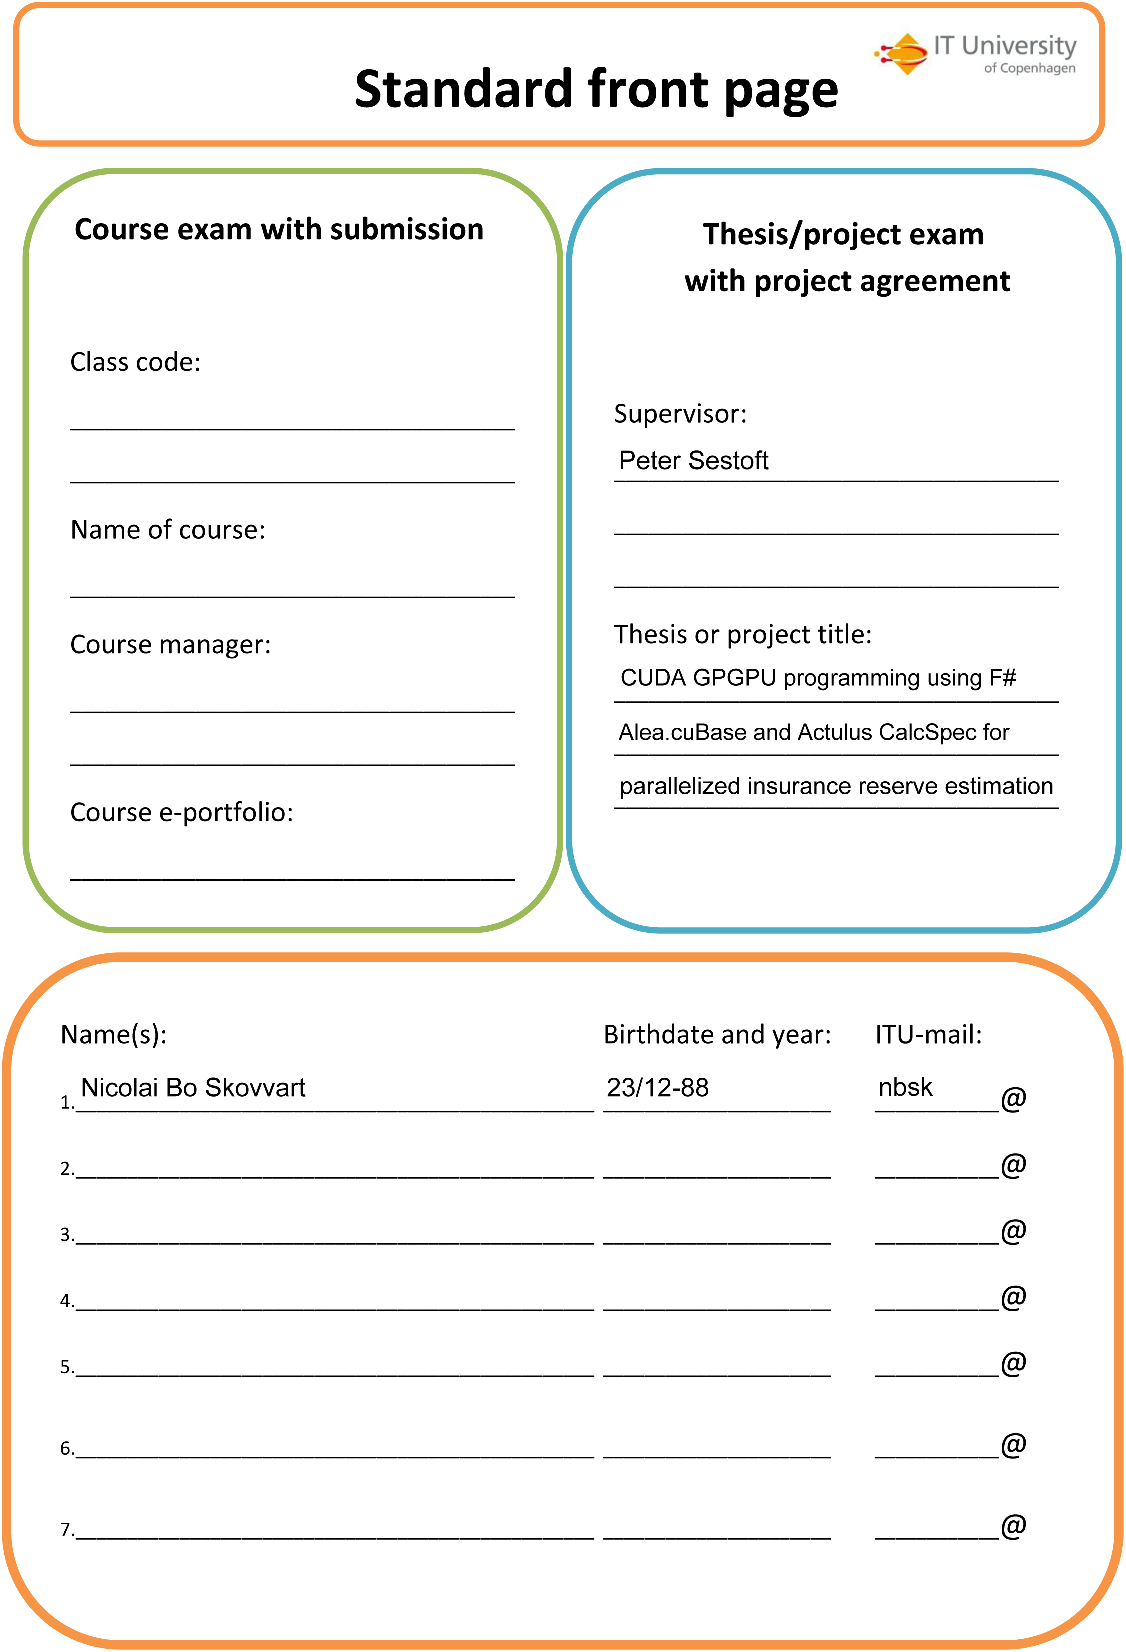
\includepdf[pages={1}]{sections/FrontPage.pdf}	
	\maketitle

	% !TeX root = ../thesis.tex
\begin{abstract}
Parallelization can provide great performance boosts for large-scale independent numerical computations, for example in the field of insurance reserve estimation.
NVIDIA's CUDA platform allows for utilization of the parallelization power of the Graphic Processing Unit, but development is traditionally done using the CUDA C language which is based on the somewhat archaic C and C++ languages.
The language integrated compiler Alea.cuBase allows for CUDA development on the .NET platform using F\#, a much more modern language, which could have many advantages for industry.

This thesis investigates the benefits of transforming a single-threaded life insurance reserve estimator to utilize GPU parallelization on the CUDA platform.
A base-line solution is implemented in CUDA C and is then ported to the F\# language with the aid of Alea.cuBase and the performance implications are explored.
The F\# solution is further enhanced with the capability of parsing life insurance plans, written in the Actulus Calculation Specification language, that are automatically transformed into GPU code using Alea.cuBase. 
The performance implications of this is also explored.
This thesis also presents work on optimizing complex life insurance models such as the collective spouse pension.

The thesis concludes that software such as insurance reserve estimators can greatly benefit from parallelization on the GPU and that the benefits of developing on a modern platform such as .NET far outweigh the costs.
The parallelized version is up to 2485 times faster than the single-threaded version allowing for vastly more computations of life insurance plans in the same amount of time.
It is also concluded that GPU code automatically transformed from calculation specifications has no noticeable loss of performance or expressiveness.
A new method for calculating the collective spouse pension was confirmed to work and provided a performance increase of factor 150 with less than 0.1\% variation in the result compared to the original method of computation.
The complexity of the model sadly only allowed for a limited implementation to run on the GPU due to issues with Alea.cuBase.

\keywords{GPU Parallelization, Language Transformation, Insurance Reserve Estimation, F\# Alea.cuBase, Actulus CalcSpec, CUDA C}
\end{abstract}
	\tableofcontents
	
	% Dirty Hack to make LoL header use section* rather than chapter* like LoF and LoT
	\newcommand\stdchapter{\chapter}
	\def\chapter*#1{\section*{#1}}
	\lstlistoflistings
	\let\chapter\stdchapter
	%End Dirty hack

	\listoffigures{}\thispagestyle{empty}
	\listoftables
	\clearpage	
	\setcounter{page}{1}
	% !TeX root = ../thesis.tex
\section{Introduction}
This thesis was written in the March-September period of 2014 at the IT University of Copenhagen (ITU) and was supervised by Peter Sestoft to whom I owe many thanks. 
I would further also like to thank all the people who have helped proof-read this thesis.
The project was performed using documentation and code provided by the Actulus project\cite{actulus}.

As the exponential growth of the Central Processing Unit (CPU) clock-rate speeds have leveled off in recent times\cite{ross2008cpu}, parallelization is seen as one of the primary techniques for increasing computational performance. 

While parallelization can be utilized by many mechanisms such as multiple machines or multi-core CPUs, General Purpose Graphics Processing Units (GPGPU's) in particular are used when computations on large amounts of data is needed. 
Despite originating from the Graphics Processing Unit (GPU) designed for performing calculations in relation to computer graphics, the parallel computing architecture is very useful in other domains.

Parallelization is especially useful for large amounts of independent calculations that can be found in financial fields such as banking or insurance.

One approach to GPGPU programming is using the Compute Unified Device Architecture (CUDA) platform by NVIDIA, which is available to most platforms, but does require an NVIDIA graphics card.
The CUDA platform supports multiple languages, including Python and Fortran, but the official and one of the most popular languages used is NVIDIA's CUDA C which is based on the somewhat archaic C and C++ languages.

In this thesis a single-threaded C\# insurance reserve estimator will be translated to the CUDA platform and parallelized and the performance ramifications will be investigated.
First a base-line implementation will be implemented in CUDA C followed by a solution implemented on the more modern .NET platform in the F\# language using the language-integrated compiler Alea.cuBase to explore the effects on performance.
If there is no significant loss of performance, this could allow for all the benefits of modern languages while also allowing GPU code to be incorporated on the .NET platform.

The thesis will also cover how insurance plans specified in the Actulus Calculation Specification language (CalcSpec) will be automatically translated to code that will run on the GPU, and the performance ramifications of this will be analysed.

Advanced life insurance plans, such as the collective spouse pension, and their relative performance impact on the GPU will also be explored.

\subsection{Reading guide}
This thesis paper is targeted at people interested in high performance and parallel computing as well as people interested in language transformation. 
Some experience with programming, especially imperative, can be considered a requirement to fully understand everything. 
A general idea of overall computer architecture will also be very useful. 
Uncommon concepts will be explained to the best of my ability. 
Experience with a variant of C and a functional language (such as F\#, an ML variant or any other) should lead to little trouble understanding the code examples.

Subjects will be described in various levels of detail depending on their relevance to the main topics of the thesis.
This means that certain technologies, languages and paradigms will be described in less detail than strictly required background information and solution descriptions.

The thesis is structured into the following sections.
The first section will introduce the thesis, including the motivation, scope, approach and methods used.

The second section will cover the required background information including life insurance policies, the math used, the technologies utilized and the hardware the code has been tested on.

The third section will cover descriptions of the various implemented solutions, starting with the initial single-threaded C\# solution followed by a CUDA C implementation. 
This is in turn followed by a solution manually written in F\# using the language integrated compiler Alea.cuBase.

The fourth section will describe how life insurance plan specifications written in Actulus CalcSpec are parsed and transformed to GPU code using F\# with Alea.cuBase and the performance ramifications of this.

The fifth section will discuss how various alterations to the project affected performance and their viability. 
These alterations include testing memory types, GPU code expression reduction and large state insurance plan models such as the collective spouse pension.

The remaining sections six through eight will discuss similarities and differences to related work, possible future work and ending with the conclusion of the thesis.
	% !TeX root = ../thesis.tex
\section{Background}
The background section will cover eight topics.
Section \ref{subsec:background:lifeinsurance} will explain insurance policies in general.
In section \ref{subsec:background:thielerungekutta} the mathematics employed in this project will be covered. 
This consists of Thiele's differential equation and the fourth-order Runge-Kutta method for solving differential equations.

After the mathematics is covered, the technologies utilized will be presented.
General information on parallelization and the potential benefits of using the GPU compared to the CPU will be explained in section \ref{subsec:background:parallelization}.
The CUDA platform and CUDA C will then be presented in section \ref{subsec:background:cudac}.
In section \ref{subsec:background:codequotations} F\#'s meta-programming model Code Quotations is introduced.
Quotations are used to generate CPU code by the language-integrated compiler Alea.cuBase which will be presented in section \ref{subsec:background:fsharpcubase}.
Section \ref{subsec:background:calcspec} will briefly introduce the syntax of the Actulus Calculation Specification (CalcSpec).
In section \ref{subsec:background:hardware} the hardware the project has been tested on will be presented.

\subsection{Life Insurance Policies and Markov-models}\label{subsec:background:lifeinsurance}
A life insurance policy is a contract stating the obligations an insuring party has to an insured party in and transitioning between a finite set of states over many years.
Such states can include being alive and well (active), disabled, dead and more.
Transitions between states will have a certain probability, for example mortality rates for transitions between the active and dead state.
A state model such as this is also known as a continuous-time Markov-model which is used for both its expressiveness and its analyzability.

Figure \ref{fig:markovexample} shows an example of such a model with 3 states and 3 transitions between states. 
The labels between the states each have a $\mu$-function that states the probability of the transition occurring at time $t$. 
This is also known as the transition intensity.
Not all transition intensities will change over time while others such as mortality rate will.
For each change in time there may be associated costs whether there is a state transition or not.

\subsubsection{Example life insurance policies}\label{subsubsec:background:insuranceplans}
The following six life insurance plan examples are used throughout the project.
\begin{itemize}
\item Pure Endowment : Ensurer pays a lump sum if the ensured dies before age of retirement. 
\item $m$-year Deferred $n$-year Temporary Life Annuity : After $m$ years, ensurer makes yearly payments to the ensured for $n$ years given the ensured is alive.
\item $n$-year Temporary Life Annuity Premium : The ensured is paid yearly for $n$ years if alive.
\item $n$-year Term Insurance : Ensurer pays a lump sum if the ensured dies before $n$ years.
\item Disability Annuity : The ensured is paid yearly for $n$ years if disabled.
\item Disability Term Insurance : Ensurer pays lump sum upon disability of ensured if it happens within $n$ years.
\end{itemize}

\begin{figure}[h] 
\setlength{\unitlength}{0.14in} % selecting unit length 
\centering % used for centering Figure 
\begin{picture}(20,8) % picture environment with the size (dimensions) 
 % 32 length units wide, and 15 units high. 
\put(3,6){\framebox(6,3){0 (Active)}} 
\put(13,6){\framebox(6,3){1 (Disabled)}}
\put(8,0){\framebox(6,3){2 (Dead)}} 

\put(6.2,6){\vector(1,-1){2.9}}
\put(9,7.5){\vector(1,0){3.9}} 
\put(16.2,6){\vector(-1,-1){2.9}}

\put(9.5,8.5) {$\mu_{01}(t)$}
\put(15,4) {$\mu_{12}(t)$} 
\put(4.5,4) {$\mu_{02}(t)$} 
\end{picture} 
\caption{Disability Term Insurance Markov-model example} % title of the Figure 
\label{fig:markovexample} % label to refer figure in text 
\end{figure} 

\subsection{Thiele's differential equation and the Runge-Kutta Method}\label{subsec:background:thielerungekutta}
The goal of the computations performed in this thesis is to estimate the amount of money (reserve) required to be able to fulfil the obligations of a given life insurance plan.
Thiele's differential equation called ``the foundation of modern life insurance mathematics''\cite{bergermathematik} is a tool for determining conditional expected values in Markov models and it can be used to express a variety of life insurance policies.
The equation is expressed below in equation \ref{eq:thiele}. It assumes continuity for $V_s$, $b_s$, $\mu$ for every $t$ and consists of the following parts:

\begin{itemize}
\item $s$ is the state
\item $V_s(t)$ is the reserve at time $t$ in state $s$
\item $r_s(t)$ is interest-rate at time $t$ in state $s$
\item $b_s(t)$ is the benefit paid by the insurer at time $t$ in state $s$
\item $T_s(t)$ is the possible transition-states from state $s$
\item $\mu_{s,ts}(t)$ is the transition intensity from state $s$ to state $ts$
\item $b_{s,ts}(t)$ is the transition cost from state $s$ to state $ts$
\end{itemize}

\begin{equation}\label{eq:thiele}
\frac{d}{dt}V_s(t) = r_s(t) V_s(t) - b_s(t) - \sum_{ts \in T_{s}} \mu_{s,ts}(t) (V_{ts}(t) - V_s(t) + b_{s,ts})
\end{equation}

To shortly summarize it, the change in reserve at time $t$ in state $s$ is the current reserve times the interest-rate minus the benefit paid by the ensurer in the state minus the weighted transitioning costs to all linked states. 
The weighted transitioning cost to a state is the intensity of the transition (probability of the transition occurring) times the difference in reserves plus the transitioning cost.

With a differential equation such as this, one way to solve it is to approximate the result numerically using the Runge-Kutta method.
The Runge-Kutta method\cite{press2007numerical} is a method for integrating ordinary differential equations (ODEs) by using a trial step at the midpoint of an interval to cancel out lower-order error terms.
It works within boundaries set by a starting and end point. 
If the starting point is greater than the end point, the algorithm works backwards with negative step-sizes.
The basic implementation uses a fixed number of steps to reduce the inaccuracy of the method. 
By increasing the number of steps, the inaccuracy of the method is reduced at the cost of increased computational costs.
The most common step size seen in this project is 100 steps by advice of Peter Sestoft and by calculation specification definitions.
The fourth-order version of the Runge-Kutta method can be seen below in equation \ref{eq:rk4} approximating $y$ in the step from $t$ to $t+h$. It consists of the following parts:

\begin{itemize}
\item $h$ is the size of the step. With 100 steps, the step-size would be 0.01, or -0.01 if the start point is greater than the end point.
\item $f(t, e)$  is the right hand side of the given differential equation evaluated at time $t$ in environment $e$
\item $t$ is the initial time of the step
\item $y_t$ approximated result at time t
\item $O(h^5)$ represents the inaccuracy of the method
\end{itemize}

\begin{equation}\begin{aligned}\label{eq:rk4}
&k_1 = h f(t, y_t)\\
&k_2 = h f(t + \frac{h}{2}, y_t + \frac{k_1}{2})\\
&k_3 = h f(t + \frac{h}{2}, y_t + \frac{k_2}{2})\\
&k_4 = h f(t + h, y_t + k_3)\\
&y_{n+1} = y_t + \frac{k_1}{6} + \frac{k_2}{3} + \frac{k_3}{3} + \frac{k_4}{6} + O(h^5)
\end{aligned}\end{equation}

%Insert graphics showing step

\subsection{Parallelization and the GPU}\label{subsec:background:parallelization}
Parallelization is the act of taking one large task and splitting it into smaller tasks that run concurrently (``in parallel'').
This could for example be cooking 10 different pies, where rather than using 1 baker you now use 10 bakers creating 10 pies at the speed of one.
Algorithmically this could be an algorithm that initially does some computation that loops $n$ times where each iteration is independent and takes $w$ time to complete, but is altered to instead utilize $n$ tasks that each execute one iteration worth of work.
Instead of taking $w \cdot n$ time to complete, it can now be done in just $w$ time plus whatever overhead is associated with creating the tasks and dividing the work.
This is reliant on each iteration being independent, as if the iterations are dependent on each other then it can not be executed before the previous iteration completes.
To continue the pie example, if one baker is assigned to make all the pie-crusts, no pie will be baked before this tasks is done.
Loops are not the only thing that can be parallelized and all independent tasks can to some extend be parallelized. 
With various synchronization techniques, partially dependent calculations can also harness the power of parallelization, though at the risk of increased complexity and errors such as deadlocks.
As only independent computation parallelization is utilized, other forms will not be discussed further.

In computing, parallelization utilizing constructs such as processes and threads can be performed on multi-core CPUs, but can especially be used by GPUs that were designed for compute-intensive and highly parallel computations, precisely what graphics rendering is about.
This is because unlike the CPU which is a general-purpose machine with a focus on data-caching and flow control, the GPU is specialized for high arithmetic processing with more transistors dedicated to data processing as illustrated in green by figure \ref{cpugpu}. 
The figure contains Arithmetic Logic Units (ALU's, in green) responsible for logical operations and integer arithmetic, Control Units (in yellow) responsible for communication and coordination between input/output devices and various memory units (in orange) such as a memory cache and dynamic random-access memory (DRAM).

\begin{figure}[h!]
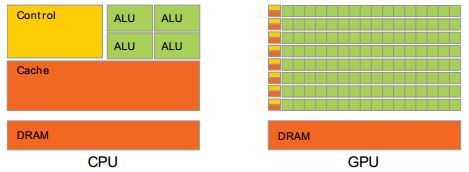
\includegraphics{cpugpu.jpg}
\caption{Structural comparison of the CPU and GPU. From the CUDA C Programming Guide, page 3 \cite{nvidia2014programming}\label{cpugpu}}
\end{figure}

\subsection{The CUDA platform and CUDA C}\label{subsec:background:cudac}
CUDA is NVIDIAs parallel computing platform and programming model for the GPU.
It is available on multiple platforms but does require an NVIDIA graphics card. 
An NVIDIA graphics card will have a certain Compute Capability (CC) that determines availability of certain attributes and features.

The CUDA platform consists of the CUDA C and C++ language (referred to as CUDA C from this point), based on the C and C++ languages but with some alterations.
It also has parallel computing extensions for other languages such as Fortran and Python.
The CUDA Toolkit is also a part of the platform, consisting of a compiler, math libraries and tools for debugging and optimizing performance as well as guides, user manuals, API references and other documentation.

\subsubsection{CUDA Architecture}
The CUDA model is build around a hierarichal architecture of the GPU. 
At the top of the architecture is the streaming multi-processor (SM) of which a GPU can have many. 
Each SM consists of multiple CUDA cores that are used to concurrently execute a group of 32 threads known as a warp. 
As the SM executes the instructions in terms of warps, the total number of threads in a block should be a multiple of the warp-size for maximum efficiency.
Each SM executes one group of threads that have access to a shared memory-space.
This group of threads, which ideally should be a multiple of warps, is called a block. 
An example overview of the architecture can be seen in figure \ref{cuda_architecture}.
As each SM executes blocks sequentially, more SMs available to the GPU will increase the possible parallelization and speed up the execution of the total amount of blocks. 
Assuming that blocks will generally finish at the same time, this also means that the amount of blocks should be a multiple of the amount of multiprocessors for maximum efficiency.

\begin{figure}[h!]\centering
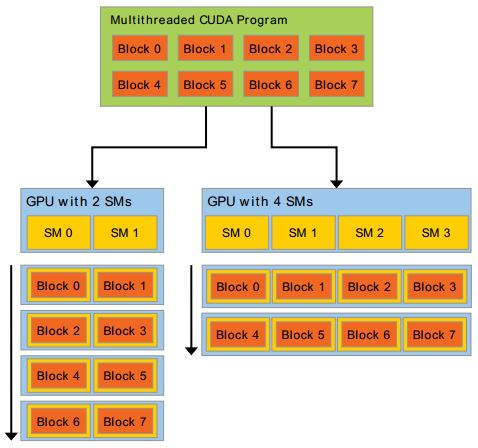
\includegraphics[scale=0.75]{cuda_architecture.jpg}
\caption{The CUDA SM/block architecture. From the CUDA C Programming Guide, page 7 \cite{nvidia2014programming}\label{cuda_architecture}}
\end{figure}

\subsubsection{Thread Hierarchy}
Blocks can be organized in a grid of multiple dimensions (up to 3 on the latest version of NVIDIA cards). 
The same applies to the threads within a block.
An example of can be seen in figure \ref{thread_distribution}.

\begin{figure}[h!]\centering
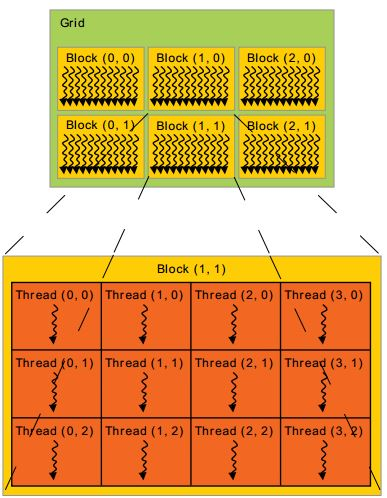
\includegraphics[scale=0.75]{thread_distribution.jpg}
\caption{The CUDA thread hierarchy. From the CUDA C Programming Guide, page 11 \cite{nvidia2014programming}\label{thread_distribution}}
\end{figure}

As this project only utilizes 1-dimensional grids and blocks, the resulting thread hierarchy is a two-dimensional matrix. 
An example with the unique thread-IDs can be seen in figure \ref{thread_hierarchy}.

\begin{figure}[h!]\centering
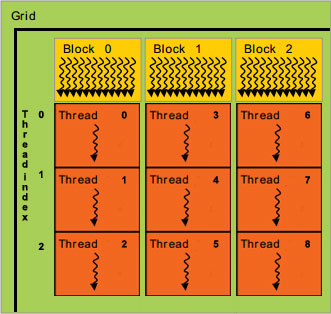
\includegraphics[scale=0.75]{thread_hierarchy.jpg}
\caption{CUDA thread hierarchy with 1-dimensional blocks and threads.\label{thread_hierarchy}}
\end{figure}


\subsubsection{Memory model}
A thread has access to various types of memory.
There is \emph{local} memory only available to the thread itself.
This is facilitated by 32KiB per block of fast registers while available and falling back on relatively slow local memory afterwards (stored in global memory but only accessed by the thread).

Beyond that, it has access to low-latency \emph{shared} on-chip memory physically residing on the GPU that is available to all threads in the same block. 
Because of these properties, shared memory can be used for communication between threads or as a software managed cache.

The thread also has access to \emph{global} off-chip memory accessible to all threads in all blocks.
This has a higher latency, but caching can alleviate some of this.

There is also 64KiB of immutable cached \emph{constant} memory which can be an alternative to unchanging global memory.
It is especially fast when all threads in the warp need to read the same memory location.
Constant memory will often be faster than global memory due to a higher likelihood of being cached on-chip, but the fact it is immutable and of a fixed size limits its applicability.
Another immutable memory type is \emph{texture} memory which can be used for various purposes, but is ideally used for algorithms with memory access patterns where threads are likely to read from an address that is 2-dimension-spatially local (such as computer graphic shaders).

Data loaded from local or global memory is cached in the on-chip \emph{L1} cache for each SM and a shared \emph{L2} cache for all SMs.
The L1 cache will typically contain up to 16KiB of data, but this limit can be increased by up to 48KiB by sacrificing shared memory size.
The L2 cache will on newer graphics cards contain up to 768KiB of data.

A summary of the properties of the various memory types can be seen in table \ref{table:memorytypes}.

\begin{table}[h!]
\centering
\begin{tabular}{ | c | c | c | c | c | }
  \hline
           & Read-only & On-chip   & Cached & Scope  \\ \hline
  Register & No        & Yes       & No     & Thread \\ \hline
  Local    & No        & No        & Yes    & Thread \\ \hline
  Shared   & No        & Yes       & No     & Block  \\ \hline
  Global   & No        & No        & Yes    & Kernel \\ \hline
  Texture  & Yes       & No        & Yes    & Kernel \\ \hline
  Constant & Yes       & No        & Yes    & Kernel \\ \hline
  L1 Cache & No        & Yes       & N/A    & N/A    \\ \hline
  L2 Cache & No        & No        & N/A    & N/A    \\ \hline

\end{tabular}
\caption{Properties of CUDA memory types\label{table:memorytypes}}
\end{table}

\subsubsection{CUDA C}
CUDA C is based on C with added declaration specifiers for methods and variables. 
The most essential declaration specifier is the \textbf{\_\_global\_\_} specifier which declares a method to be a \textbf{kernel}. 
Kernels are void-methods that are callable from the CPU but executed on the GPU. 
Code sample \ref{cuda_add} shows a simple kernel performing vector addition of the vectors $a$ and $b$ of size $N$.

\begin{lstlisting}[language=C++, caption=CUDA C addition kernel, label=cuda_add]
__global__ void Add(float *a, float *b, float *result){
	//unique id within the kernel
	int i = threadIdx.x + blockIdx.x * blockDim.x;
	// (blockIdx always 0 in this example)
	result[i] = a[i] + b[i];
}

int main(){
	...Initiate memory on host and device
	Add<<<1, N>>>(a, b, result); //run kernel on 1 block of N threads
	...Copy back and use result, free memory as appropriate
}
\end{lstlisting}

One thing to note is the kernel launch-parameters of Add-method in $main$ which specify the number of blocks and the number of threads per block on which the kernel should be executed. 

CUDA C also has other declaration specifiers. 
The \textbf{\_\_device\_\_} specifier indicates that a method will only be compiled for the GPU (which can be referenced by kernels), the \textbf{\_\_host\_\_} specifier indicates that a method will be available for the CPU.
These two specifiers can also be used together for compilation to both platforms.
Variables also have the \textbf{\_\_device\_\_} specifier, as well as the \textbf{\_\_constant\_\_} specifier to indicate that they are to be stored in constant memory and the \textbf{\_\_shared\_\_} specifier for shared memory.

As it is based on C, dynamic memory must be allocated using $malloc$ and subsequently de-allocated by $free$.
This operation also has to be done for the device memory using the equivalent $cudaMalloc$ and $cudaFree$.
One of the many benefits of using a modern language is avoiding tedious memory management like this, but at the cost of control that could potentially decrease performance.

\subsection{F\# and Code Quotations}\label{subsec:background:codequotations}
F\#\cite{fsharp} is an open source, cross-platform functional programming language originating from Microsoft that runs on the .NET platform.
Code Quotations is a language feature of F\# that allows one to dynamically generate abstract syntax trees from F\# expressions. 
It is used in particular to transform F\# to other languages such as SQL automatically. 
It can also be used to generate F\# code that can be evaluated. 
Code Quotations support both typed and untyped expressions using \emph{\textless @ ... @\textgreater} and \emph{\textless @@ ... @@\textgreater} respectively. 

For example, the expression \emph{\textless @ let plusfive number = number + 5 in plusfive @\textgreater} is automatically translated into the abstract syntax tree in figure \ref{quotationast}. 
As Quotations only support expressions, a let declaration can not exist on its own, hence returning the function at the end (in the $in$ part of the Quotation).

\begin{lstlisting}[caption=Abstract syntax tree for the example Quotation expression, label=quotationast]
Let (plusfive, 
	Lambda (number, 
		Call (None, op_Addition, [number, Value (5)])
	), 
	plusfive)
\end{lstlisting}

Code Quotations also allow for the mixing of Quotation expressions using the splicing operators $\%$ for typed and $\%\%$ for untyped expressions as can be seen in code sample \ref{quotationsmixin}.

\begin{lstlisting}[caption=Quotation mixing, label=quotationsmixin, language=ml]
let plusfive = <@ let plusfive number = number + 5 in plusfive @>
//Has type Expr<int->int>
let plus10 = <@ let plusten number = number |> %plusfive |> %plusfive in plusten @>
//Also has type Expr<int->int>
let untypedplus10 = <@@ %plus10 @@>
//Has type Expr
\end{lstlisting}


\subsection{F\# and Alea.cuBase}\label{subsec:background:fsharpcubase}
Alea.cuBase by QuantAlea\cite{quantalea} is a commercial language-integrated compiler for F\# that allows for CUDA development on the .NET platform.
By relying on run-time code-generation it allows for extremely extensible kernels to an extent not easily possible in CUDA C.

It utilizes F\#'s meta-programming support Code Quotations for automatic run-time generation of abstract syntax-trees that are then compiled into CUDA's Instruction Set Architecture (ISA) Parallel Thread Execution (PTX) code using Alea.cuBase's compilation API.
Code sample \ref{cubase_add} shows what a simple vector squaring-kernel could look like in F\# using Alea.cuBase.

\begin{lstlisting}[caption=Alea.cuBase square kernel, label=cubase_add, language=ml]
let Square = cuda { //use the Alea.cuBase cuda workflow
  let! kernel = <@ fun (a:deviceptr<int>) (result:deviceptr<int>) ->
      let i = blockIdx.x * blockDim.x + threadIdx.x
      result.[i] <- a.[i] * a.[i] @> |> Compiler.DefineKernel
  return Entry(fun program ->
    let worker = program.Worker
    let kernel = program.Apply kernel
    //return host-execution method
    fun (a:int[]) ->
      use a = worker.Malloc(a)
      use result = worker.Malloc(Array.zeroCreate a.Length)
      kernel.Launch (LaunchParam(1, a.Length)) a.Ptr result.Ptr
      result.Gather()) //return result
}
[<EntryPoint>]
let main argv = 
  let a = [| for i in 1 .. 10 -> i |]
  use program = Square |> Compiler.load Worker.Default
  program.Run a |> Array.iter (fun e -> printfn "%d" e)
  0 //return 0 to indicate success
\end{lstlisting}

The $cuda$ workflow/computation expression (or ``monad'' for the so inclined) contains the kernel defined in a Code Quotation and compiled to an actual kernel, and it returns a host-side execution method that will handle allocation and de-allocation of device-side memory. 
As we are using F\#, the deallocation is handled automatically by using the $use$-keyword that automatically frees up resources once the variables referencing them are out of scope. 
The kernel is loaded to a worker (a CUDA context and background-thread) in the main method compiling the PTX code to NVIDIA internal ISA code. %explain better
Following this, the compiled kernel is run using the parameters defined in the run-time method of the $cuda$ workflow (in this case, just an integer array) and the result is returned to the CPU where it can be processed. 
In this example is it simply printed to the console. 

\subsection{Actulus Calculation Specification language}\label{subsec:background:calcspec}
The Actulus Calculation Specification language (CalcSpec) is a domain-specific language for defining the differential equations that make up an insurance plan.
The main purpose of the language is to define various coefficient used in the Markov-model defining the life insurance policy.
The overall structure of the language can be seen in code sample \ref{calcspecstructure}.

\begin{lstlisting}[caption=CalcSpec structure, label=calcspecstructure, language=calcspec]
calculation = {
    name = <Name of calculation>,
    algorithm = { <Algorithm> },
    equations = { <Equations> },
    range = { <Range> },
    [output = "[" <Output> "]",]
    boundaryvalues = { <Boundary values> },
    expressions = { <Expressions> }
  }
\end{lstlisting}

An explanation of each element follows:
\begin{itemize}
\item The \textless Algorithm\textgreater{} will include the name of the algorithm (for example ``Runge Kutta 4'') and the parameters (for example the step-size for Runge Kutta 4) for the algorithm.
\item The \textless Equations\textgreater{}  describes the differential equations used by the algorithm. This is typically done by referencing functions defined in \textless{}Expressions\textgreater{}. Every component of the differential equation must describe the coefficients of the component. If coefficients are 0, they can also be described as constants (for example 0) or as an empty block for multi-part coefficients.
\item The \textless{}Range\textgreater{} and \textless{}Boundary values\textgreater{} are related to the differential equation described in \textless{}Equations\textgreater{} and describes the interval in which the algorithm should solve the equation subject to the boundary conditions.
\item \textless{}Output\textgreater{} is an optional declaration that specifies which parts of the calculations that should be returned. It is currently not supported in this project. %Update if added
\item \textless{}Expressions\textgreater{} is where constants and function are defined. Functions can only take one parameter but can reference other constants and variables.
\end{itemize}

An example of the pure endowment insurance plan can be seen in code sample \ref{pe_calcspec}. 
Note that it utilizes the Dirac $delta$ function\cite{hassani2009dirac} which is used to express a discontinuity point in which a lump sum is to be paid.%confirm this isn't bullshit


\begin{lstlisting}[caption=The pure endowment insurance plan expressed in CalcSpec, label=pe_calcspec, language=calcspec]
calculation = 
  {
    name = 'Pure endowment',
    algorithm = { type = 'Runge Kutta 4', parameters = { stepsize = 0.01 } },
    equations = { 
        0 = { r_j = r, b_j = b0, mu_jk = { 1 = GM }, b_jk = { } },
        1 = { },
    },
    range = { from = 40, to = 0 },
    boundaryvalues = { 0 = 0 , 1 = 0 },
    expressions = {
        interestrate = 0.05,
        bpension = 1,
        pensiontime = 35,
        age = 30,
        r(t) = interestrate,
        b0(t) = bpension * delta(t - pensiontime),
        GM(t) = 0.0005 + 10 ^ (5.728 - 10 + 0.038*(age + t))
    }
  }
\end{lstlisting}

\subsection{Hardware}\label{subsec:background:hardware}
As the intended audience for this particular application of parallelization is fairly limited and can be expected to afford specific hardware, it has not been a concern that specific hardware may be required to run it.
That being said, the minimal requirement to run the program is only an NVIDIA GPU of at least compute capability 2.0 as it is the minimal requirement to use Alea.cuBase (and use double-precision floats).
The code was only tested on the NVIDIA Tesla C2075 GPU which has the following properties (see appendix \ref{app:deviceQuery} for full results of running NVIDIA's deviceQuery tool):

\begin{itemize}
\item Compute capability: 2.0
\item Multiprocessors: 14
\item CUDA cores per Multiprocessor: 32
\item GPU Clock rate: 1147 MHz (1.15 GHz)
\item Memory clock rate: 1566 MHz
\item Total global memory: 4.096GB
\item Total constant memory: 64KiB
\item Total shared memory per block: 48KiB
\item Total amount of registers per block: 32KiB
\item Total amount of threads per multiprocessor: 1536
\item Total amount of threads per block: 1024
\item L2 Cache Size: 768KiB
\item Run time limit on kernels: No
\end{itemize}

The CPU is a 2.53GHz Intel Xeion W3505 and the system has 4GB ram.

	\section{Solutions}
	% !TeX root = ../thesis.tex
%The required reserve will increase with age, and likelihood of death, until retirement is reached in which no reserve will be needed.
\subsection{Initial C\# Solution}
The original solution was single-threaded and written in C\# by Peter Sestoft using various optimizations (such for example using $Exp$ rather than $Pow$. 
It features 6 life insurance plans and multiple implementation of Runge-Kutta solvers. 
The insurance plans are the following:
\begin{itemize}
\item Pure Endowment : Ensurer pays a lump sum if the ensured dies before age of retirement. 
\item $m$-year Deferred $n$-year Temporary Life Annuity : After $m$ years, ensurer makes yearly payments to the ensured for $n$ years if the ensured is alive.
\item $n$-year Temporary Life Annuity Premium : The ensured is paid yearly for $n$ years if alive.
\item $n$-year Term Insurance : Ensurer pays a lump sum if the ensured dies before $n$ years.
\item Disability Annuity : The ensured is paid yearly for $n$ years if disabled.
\item Disability Term Insurance : Ensurer pays lump sum upon disability of ensured if it happens within $n$ years.
\end{itemize}

The plans are implemented using C\# classes without inheritance or the like, as they attempt to stay relatively similar to a potential C-solution.

The Runge-Kutta 4 solver introduced last is the fastest and is an imperative version which reuses intermediary arrays.
It has the following signature: \textit{static double[][] RK4\_n(Action\textless double, double[], double[]\textgreater  dV, Action\textless double, double[]\textgreater  bj\_ii, int a, int b, int steps, double[] Va)}.
The $dV$ function implements an arbitrary amount of derivatives.
The $bj\_ii$ function is used for lump-sum payments.
$a$ and $b$ are start and end points respectively, $steps$ are the amount of steps to use in Runge-Kutta 4 and $Va$ is the initial reserve (at time $a$).

An example implementation of the Pure Endowment life insurance plan can be seen below in code sample \ref{csharp_pureendowment}. 
Note: It does refer to some shared constants and methods defined outside the class itself.

\begin{lstlisting}[caption=The pure endowment insurance plan expressed in C\#, label=csharp_pureendowment]
class PureEndowment{
    static double b_0(double t){ return 0.0;}
    static double mu_01(double t){ return GM(t); }
    static double bj_00(double t){ return t == pensiontime ? bpension : 0.0; }
    static double bj_01(double t){ return 0.0; }
    public static double[][] Compute(){
        return RK4_n(
            (double t, double[] V, double[] res) => { 
                res[0] = r(t) * V[0] - b_0(t) - mu_01(t) * (0 - V[0] + bj_01(t)); 
            },
            (double t, double[] res) => { res[0] = bj_00(t); },
            40, 0, steps, new double[] { 0 });
    }
}
\end{lstlisting}

Using floating point numbers of 32-bit precision (floats) it could do one iteration of all six plans in approximately \emph{25.3} milliseconds (ms), and with 64-bit precision (doubles) it took approximately \emph{24.5} ms on the test machine.
It may look surprising that the float-version was actually slowe.
This is in part due to the fact that the $Exp$ function from System.Math uses and returns doubles (and requires type-casting), but is mainly because double operations are optimized by the hardware\cite{northrup2008mcts}.
The float version should have an edge if the application was memory-bound, but this is not the case in this situation.
	% !TeX root = ../thesis.tex
\subsection{CUDA C Solution}
A CUDA C solution was implemented to be used as a base-line comparison for further development.
It is intended to be fairly efficient but not much time has been spent optimizing it, as this has never been the end-goal.
It is based on the initial C\# solution but has some alterations due to the language.
It features the same 6 life insurance plans as the C\# version, but a key difference is that every plan has its own implementation of a Runge-Kutta 4 kernel which is identical but for references to implementations of different $dV$ and $bj\_ii$ functions and the number of states used by the plan.
This is due to the CUDA C kernels not allowing references to objects or methods. %unless certain version of cuda?
Another difference is that all of the kernel code is required to be in the same file as no cross-referencing is possible unlike the C\# version.

See code sample \ref{cuda_pureendowment} for an implementation of Pure Endowment in CUDA C.
\begin{lstlisting}[language=cudac, caption=The pure endowment insurance plan expressed in CUDA C, label=cuda_pureendowment]
__device__ class PureEndowment {
	__device__ floatP b_0(floatP t) { return (floatP)0; }
	__device__ floatP mu_01(floatP t) { return GM(t); }
	__device__ floatP bj_00(floatP t) { return t == pensiontime ? bpension : (floatP)0; }
	__device__ floatP bj_01(floatP t) { return (floatP)0; }
public:
	#define PESTATES 1
	__device__ void dV(floatP t, floatP* V, floatP* res){ 
		res[0] = r(t) * V[0] - b_0(t) - mu_01(t) * (0 - V[0] + bj_01(t));
	}

	__device__ void bj_ii(floatP t, floatP* res){
		res[0] = bj_00(t);
	}
} pe;
\end{lstlisting}

Note that this code uses the $floatP$ type alias to easily switch between float and double precision.
What may be of interest is the that the $pe$ object is copied to device memory and that a compile-time replaced $PESTATES$ macro is defined.
The device-size object is then referenced in the plan-specific implementation of the Runge-Kutta 4 solver.
The macro is due to C/C++ requiring constant values for array initialization.
Dynamic memory allocation and deallocation of the temporary arrays could be used, but testing showed that it had a significant negative implication on the runtime, especially at higher thread and block configurations.

The results of running one iteration with 32-bit float precisions took 42,0 ms, about 65\% slower than the C\# equivalent.
The double-precision took 124,48, or about 500\% times slower than the C\# equivalent.
The key factor to consider is the fact that the parallelized version was never intended to be faster with one iteration.
Where the single-threaded version scales linearly with the amount of iterations, the parallelized version scales much better.

The highest performance tested with float precision was at 91,43 iterations per millisecond, making it more than 2200 times faster than the C\# version.
The highest performance with double precision was at 25,97 iterations per millisecond, making it more than 650 times faster than the C\# version.
The double precision version, while respectable, was a good bit slower than could be expected and could most likely be optimized to a rate where it would be about half as fast as the float precision equivalent.

For the full float results see table \ref{table:cudacfloattime} and for double results see table \ref{table:cudacdoubletime}.
What may be of interest is the diagonals where the total thread amount ($blocks \cdot threads$) is the same.
Here a trend can be spotted where increasing the thread amount appears to be preferable to increasing the block amount, though not by a large factor.

For the full CUDA C performance comparisons, see appendix \ref{app:cuda_runtimes}


\begin{table}[h!]
\centering
\begin{tabular}{ | c | c | c | c | c | c | c | c | c | }
  \hline
           & Blocks &  1    &   14  & 14*5  & 14*10 & 14*20 & 14*25 & 14*30 \\ \hline
  Threads  &        &       &       &       &       &       &       &       \\ \hline
  1        &        & 0,02  & 0,33  & 1,55  & 1,56  & 2,00  & 1,92  & 2,17  \\ \hline
  8        &        & 0,19  & 2,65  & 12,39 & 12,45 & 15,94 & 15,35 & 17,35 \\ \hline
  16       &        & 0,38  & 5,28  & 24,69 & 24,81 & 31,58 & 30,59 & 34,61 \\ \hline
  32       &        & 0,75  & 10,48 & 49,02 & 49,26 & 63,16 & 60,76 & 68,91 \\ \hline
  64       &        & 1,47  & 20,58 & 64,17 & 70,13 & 81,71 & 80,77 & 86,85 \\ \hline
  128      &        & 2,62  & 35,83 & 72,14 & 80,42 & 83,14 & 85,78 & 85,69 \\ \hline
  256      &        & 3,20  & 44,15 & 78,57 & 90,82 & 91,07 & 88,55 & 89,01 \\ \hline
  512      &        & 12,16 & 45,49 & 91,03 & 91,35 & 91,41 & 91,40 & 91,43 \\ \hline
\end{tabular}
\caption{CUDA C calculations per ms with float precision\label{table:cudacfloattime}}
\end{table}


\begin{table}[h!]
\centering
\begin{tabular}{ | c | c | c | c | c | c | c | c | c | }
  \hline
           & Blocks &  1   &   14  & 14*5  & 14*10 & 14*20 & 14*25 & 14*30 \\ \hline
  Threads  &        &      &       &       &       &       &       &       \\ \hline
  1        &        & 0,01 & 0,11  & 0,51  & 0,50  & 0,65  & 0,61  & 0,69  \\ \hline
  8        &        & 0,06 & 0,90  & 4,06  & 4,01  & 5,16  & 4,89  & 5,50  \\ \hline
  16       &        & 0,13 & 1,79  & 8,11  & 8,02  & 10,33 & 9,77  & 11,01  \\ \hline
  32       &        & 0,26 & 3,59  & 16,22 & 16,03 & 20,65 & 19,53 & 22,01 \\ \hline
  64       &        & 0,51 & 6,94  & 18,49 & 21,71 & 23,59 & 24,10 & 25,12 \\ \hline
  128      &        & 1,00 & 11,52 & 22,74 & 25,00 & 25,30 & 25,25 & 25,69 \\ \hline
  256      &        & 1,67 & 12,98 & 25,55 & 25,59 & 25,93 & 25,88 & 25,97 \\ \hline
  512      &        & 1,85 & 25,95 & 25,96 & 25,97 & 25,97 & 25,97 & 25,97 \\ \hline
\end{tabular}
\caption{CUDA C calculations per ms with double precision\label{table:cudacdoubletime}}
\end{table}
	% !TeX root = ../thesis.tex
\subsection{F\# Alea.cuBase Solution}
The F\# Alea.cuBase solution has many similarities to the CUDA C implementation.
One key factor is that the Runge-Kutta four kernel is implemented using Code Quotations (see section \ref{subsec:background:codequotations}), as are the plan-specific $dV$ and $bj\_ii$ methods.
As the plan-specific $dV$ and $bj\_ii$ typically include references to helper-methods, they could be defined in terms of Quotations and referenced using the splicing operators.
Another option is to use use the \lstinline$[<ReflectedDefinition>]$ F\# attribute on methods which make most regular methods accessible in Quotations.
An example of this can be seen in code sample \ref{cubase_pureendowment}. 
The various plans are in this case not implemented using classes (though they could have been), so each method name is prepended with a plan acronym ($pe\_$).
It also refers to some constants and methods not defined in the class similar to previous implementations.
%\clearpage
\begin{lstlisting}[language=FSharp, caption=The pure endowment insurance plan expressed in F\# Alea.cuBase, label=cubase_pureendowment]
[<ReflectedDefinition>] 
let pe_b_0 t = zero
[<ReflectedDefinition>]
let pe_mu_01 t = GM t
[<ReflectedDefinition>]
let pe_bj_00 t = if t = pensiontime then bpension else zero
[<ReflectedDefinition>]
let pe_bj_01 t = zero
let pe_dV = 
  <@ fun t (V:deviceptr<floatP>) (res:deviceptr<floatP>) -> 
      res.[0] <- r t * V.[0] - pe_b_0 t - pe_mu_01 t * (zero - V.[0] + pe_bj_01 t) @>
let pe_bj_ii = 
  <@ fun t (res:deviceptr<floatP>) ->
      res.[0] <- pe_bj_00 t @>
\end{lstlisting}

To run the plan there is one Runge-Kutta four kernel defined, which can be be seen partially in code sample \ref{cubase_rk4_n_snippet}. 
For the full implementation see appendix \ref{app:cubase_rk4_n}. 
What may be of interest is the $deviceptr$ type used by $Va$ and $result$, which works very similarly to pointers in C and C++.
The temporary arrays $k_i$, $tmp$ and $v$ may also be of interest. 
They are initiated using Alea.cuBase and then transformed into the generic $deviceptr$ type representations like $Va$ and $result$.
%\clearpage
\begin{lstlisting}[language=FSharp, caption=The Runge-Kutta four solver expressed in F\# Alea.cuBase, label=cubase_rk4_n_snippet]
let RK4_n dV bj_ii states = cuda {
	let! kernel =
		<@ fun a b steps (Va:deviceptr<floatP>) (result:deviceptr<floatP>) ->
			//Calculate unique result offset
			let offset = (blockIdx.x * blockDim.x + threadIdx.x) * states * (a + 1)
            //Splice in other quotation expressions
			let dV = %dV
			let bj_ii = %bj_ii
			let h   = -one / conv steps
			//Initialize reusable intermediary arrays
			let k1	  = __local__.Array<floatP>(states) |> __array_to_ptr
			let k2	  = __local__.Array<floatP>(states) |> __array_to_ptr
			let k3	  = __local__.Array<floatP>(states) |> __array_to_ptr
			let k4	  = __local__.Array<floatP>(states) |> __array_to_ptr
			let tmp	  = __local__.Array<floatP>(states) |> __array_to_ptr
			let v	  = __local__.Array<floatP>(states) |> __array_to_ptr
            ...Actual Runge-Kutta 4 implementation
        @> |> Compiler.DefineKernel 

    return Entry(fun program ->
        let worker = program.Worker
        let kernel = program.Apply kernel
        fun a b steps blocks threads ->
            //Calculate size of result array
            let n = (a + 1) * states * blocks * threads
            //Allocate memory on device
            use Va = worker.Malloc<floatP>(Array.zeroCreate states)
            use result = worker.Malloc<floatP>(Array.zeroCreate n)
            let lp = LaunchParam (blocks, threads)
            ...Timing mechanism start
            //Launch kernel with parameters
            kernel.Launch lp a b steps Va.Ptr result.Ptr
            ...Timing mechanism end, save kernel execution time in ms
            //Gather and return device results and kernel execution time
            let result = result.Gather()
            result, ms
        )
}
\end{lstlisting}

As the GPU code is generated at runtime, a lot of the compile-time limitations of CUDA C disappear.
While the kernels may not take all types of parameters at launch-time, during kernel-compilation they can often be used.
The code is not making use of the functional programming paradigm and memory-allocation for the device is still required.
There are however many small changes like the $use$ keyword, and not having to provide the size of the allocated memory, still make it faster and safer to program in F\# as opposed to CUDA C.

The solution also makes use of a method to compile the kernels for reuse and another to execute them, as can be seen in code sample \ref{cubase_compileandrun}. 

\begin{lstlisting}[language=FSharp, caption=Kernel compilation and execution methods in F\# Alea.cuBase, label=cubase_compileandrun]
let compile dV bj_ii states = RK4_n dV bj_ii states |> Compiler.load Worker.Default

let runKernel (program:Program<int->int->int->int->int->floatP[]*float>) a b blocks threads = program.Run a b steps blocks threads
\end{lstlisting}

The results of running the F\# Alea.cuBase solution shows that the highest number of calculations per ms were \emph{98.33} for single precision and \emph{25.30} per ms for double precision.
For the full single-precision results table \ref{table:cubaseManualfloattime} and for double precision results see table \ref{table:cubaseManualdoubletime}.
For the entire results, see appendix \ref{app:cuBase_manual_runtimes}.
This is a slight improvement over the CUDA C single precision version while being nearly identical for double precision.
%Unlike the CUDA C version, I was not able to limit the maximum amount of registers used, making it impossible to test configurations with more than 512 threads.
The documented way to limit the maximum number of registers in Alea.cuBase did not work, so it was impossible to run double precision configurations with 1024 threads.

For more information on result comparison see section \ref{subsec:result_comparison}.

\begin{table}[h!]
\centering
{\setlength{\extrarowheight}{2pt}{\setlength{\tabcolsep}{3pt}
\begin{tabular}{ | r | r | r | r | r | r | r | r | }
  \hline
\diaghead{Threads/Blocks}{Threads}{Blocks}
		&	1		& 	14 	 	&	14*5 	& 	14*10 	& 	14*20 	& 	14*25 	& 	14*30 	\\ \hline
1		& 	0.02	&	0.34 	&	1.61	&	1.67	&	2.15	&	2.04	&	2.36	\\ \hline
8		& 	0.19	&	2.72 	&	12.87	&	13.33	&	17.13	&	16.28	&	18.80	\\ \hline
16		&	0.38	&	5.43	&	25.60	&	26.53	&	34.05	&	32.35	&	37.47	\\ \hline
32		&	0.76	&	10.78	&	50.58	&	52.59	&	67.61	&	64.27	&	74.51	\\ \hline
64		&	1.37	&	21.12	&	67.15	&	70.75	&	88.71	&	85.95	&	95.53	\\ \hline
128		&	1.69	&	37.36	&	77.74	&	84.81	&	85.36	&	88.89	&	92.55	\\ \hline
256		&	1.73	&	46.54	&	95.53	&	97.41	&	97.92	&	94.80	&	95.49	\\ \hline
512		&	6.75	&	48.20	&	97.44	&	98.01	&	98.23	&	96.28	&	98.31	\\ \hline
1024	&	6.93	&	96.11	&	97.94	&	98.16	&	98.31	&	98.33	&	98.29	\\ \hline
\end{tabular}}}
\caption{F\# Alea.cuBase calculations per ms with single precision\label{table:cubaseManualfloattime}}
\end{table}

\begin{table}[h!]
\centering
{\setlength{\extrarowheight}{2pt}{\setlength{\tabcolsep}{3pt}
\begin{tabular}{ | r | r | r | r | r | r | r | r | }
  \hline
\diaghead{Threads/Blocks}{Threads}{Blocks}
		&	1		&	14		&	14*5	&	14*10	&	14*20	&	14*25	&	14*30	\\ \hline
1		&	0.01	&	0.11	&	0.49	&	0.49	&	0.63	&	0.59	&	0.69	\\ \hline
8		&	0.06	&	0.87	&	3.93	&	3.91	&	5.01	&	4.74	&	5.51	\\ \hline
16		&	0.12	&	1.73	&	7.83	&	7.88	&	10.05	&	9.48	&	11.01	\\ \hline
32		&	0.25	&	3.46	&	15.63	&	15.75	&	20.06	&	18.94	&	22.02	\\ \hline
64		&	0.49	&	6.73	&	19.96	&	21.67	&	24.42	&	23.22	&	25.22	\\ \hline
128		&	0.96	&	11.26	&	20.31	&	25.18	&	24.10	&	24.94	&	25.34	\\ \hline
256		&	1.61	&	12.53	&	24.84	&	25.12	&	25.27	&	25.35	&	25.42	\\ \hline
512		&	1.79	&	25.03	&	25.26	&	25.28	&	25.30	&	25.30	&	25.25	\\ \hline
\end{tabular}}}
\caption{F\# Alea.cuBase calculations per ms with double precision\label{table:cubaseManualdoubletime}}
\end{table}

\subsection{Insurance plan parameterization}\label{sub:manual_parameterization}
The parallelized versions have so far been running the same static plans repeatedly which is not very useful in practical scenarios.
To make parallellisation useful, the ability to replace constants with parameters is required.
For example, a constant could be the interest rate for the insurance plan or the age of the insured.

To add this parameterization, the $dV$ and $bj\_ii$ method signatures were changed to include an additional array containing parameters for the insurance plan.
The life insurance plan implementations were then made responsible for knowing how many variables there were and which variables mapped to which position in the parameter array. 
They also had to pass the parameters to the methods that required them, for example the age to the mortality functions.
This iteration of the code also switched to using classes eliminating the need for prepending prefixes to the various plan methods.
For an example of this, see code sample \ref{cubase_pureendowmentparams}.
The RK4\_n kernel was also altered to provide the thread-specific pointer to the plan parameter array and pass this to the updated $dV$ and $bj\_ii$ methods.
This position would be the position of the thread multiplied by the number of plan parameters.
For a brief overview of the changes to the RK4\_n kernel, see code sample \ref{cubase_rk4nparams}.
%\clearpage
\begin{lstlisting}[language=FSharp, caption=Parameterized pure endowment life insurance plan in F\# Alea.cuBase, label=cubase_pureendowmentparams]
type PureEndowment (planParams, paramCount) =
  inherit Plan<floatP>(40, 0, 1, planParams, paramCount) with
    [<ReflectedDefinition>]
    let b_0 t = conv 0
    
    [<ReflectedDefinition>]
    let mu_01 t age = GM t age
    
    [<ReflectedDefinition>]
    let bj_00 t pensiontime bpension = if t = pensiontime then bpension else conv 0

    [<ReflectedDefinition>]
    let bj_01 t = conv 0

    override this.dV = <@ fun t (V:deviceptr<floatP>) (planParams:deviceptr<floatP>) (res:deviceptr<floatP>) -> 
      let age = planParams.[0]
      res.[0] <- (r t) * V.[0] - (b_0 t) - (mu_01 t age) * (conv 0 - V.[0] + (bj_01 t))
      @>
    override this.bj_ii = <@ fun t (planParams:deviceptr<floatP>) (res:deviceptr<floatP>) -> 
      let bpension = planParams.[1]                
      let pensiontime = planParams.[2]
      res.[0] <- bj_00 t pensiontime bpension
      @>
\end{lstlisting}

\begin{lstlisting}[language=FSharp, caption=Parameterized RK4\_n kernel changes in F\# Alea.cuBase, label=cubase_rk4nparams]
let RK4_n (plan:Plan<_>) = cuda {
  let! kernel =
    <@ fun (a:int) b steps (Va:deviceptr<floatP>) (d_params:deviceptr<floatP>) (result:deviceptr<floatP>) ->
      if blockIdx.x * blockDim.x + threadIdx.x > plan.planParams.Length/plan.paramCount then () else

      let localParams = d_params.Ptr ((threadIdx.x + blockIdx.x*blockDim.x)*plan.paramCount)
      while y > b do
        bj_ii (conv y) localParams v
        for s = 0 to steps - 1 do
          dV (if s = 0 then t - limit else t) v localParams k1
          dV (t + h / conv 2) tmp localParams k2
          dV (t + h / conv 2) tmp localParams k3
          dV (if s = steps - 1 then t + h + limit else t + h) tmp localParams k4
        y <- y - 1
    @> |> Compiler.DefineKernel 

  return Entry(fun program ->
    fun a b steps blocks threadsPerBlock ->
      use planParams = worker.Malloc<'T>(plan.planParams)
      let msec, _ = time false "" (fun () -> kernel.Launch lp a b steps Va.Ptr planParams.Ptr result.Ptr)
    )
}
\end{lstlisting}
%\clearpage
The parameters were shaped so each thread would have its own unique set of parameters laid in sequence. 
See figure \ref{fig:ParameterizationVisualization} for a visualized example of this.

\begin{figure}[h!]\centering
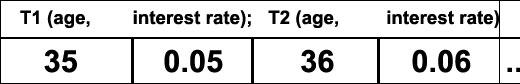
\includegraphics[scale=0.4]{ParameterizationVisualization.jpg}
\caption{Parameterization visualization for the variables age and interest rate for threads T1 and T2.\label{fig:ParameterizationVisualization}}
\end{figure}

Results were slightly slower for floats with the highest number of calculations per second being \emph{95.26} calculations per ms, but almost twice as fast for doubles with \emph{54.53} calculations per ms. 
For the remaining iterations per ms results see tables \ref{table:cubaseManualParamsfloattime} and \ref{table:cubaseManualParamsdoubletime} for single and double precision respectively.
For the runtimes see appendix \ref{app:cuBase_manual_params_runtimes}.
The performance increase in the double precision results are likely because less of the functions rely on constants defined outside the functions themselves, instead relying on passing the parameters to the function. %this explanation is still shit
This is likely something that can be used for further projects. %test this

The results of the test shows that parameters not only barely affect the running time and are therefore more than viable, it also shows that the double results in particular can be optimized a good bit which increases their viability significantly.

\begin{table}[h!]
\centering
{\setlength{\extrarowheight}{2pt}{\setlength{\tabcolsep}{3pt}
\begin{tabular}{ | r | r | r | r | r | r | r | r | } \hline
\diaghead{Threads/Blocks}{Threads}{Blocks}
	&	1		&	14		&	14*5	&	14*10	&	14*20	&	14*25	&	14*30	\\ \hline
1	&	0.02	&	0.32	&	1.53	&	1.60	&	2.09	&	1.99	&	2.33	\\ \hline
8	&	0.19	&	2.59	&	12.17	&	12.70	&	16.56	&	15.80	&	18.30	\\ \hline
16	&	0.37	&	5.13	&	24.07	&	25.09	&	32.71	&	31.29	&	36.43	\\ \hline
32	&	0.71	&	10.00	&	46.89	&	48.79	&	63.86	&	60.94	&	70.47	\\ \hline
64	&	1.43	&	19.66	&	62.13	&	69.81	&	85.64	&	82.79	&	90.86	\\ \hline
128	&	2.82	&	34.63	&	70.70	&	68.48	&	90.20	&	86.77	&	92.09	\\ \hline
256	&	5.09	&	43.36	&	82.92	&	87.60	&	94.94	&	94.27	&	94.98	\\ \hline
512	&	6.37	&	45.93	&	94.01	&	93.44	&	95.28	&	94.93	&	95.38	\\ \hline
1024&	6.64	&	92.45	&	94.76	&	95.06	&	95.22	&	95.26	&	95.24	\\ \hline
\end{tabular}}}
\caption{F\# Alea.cuBase calculations per ms with single precision and parameters\label{table:cubaseManualParamsfloattime}}
\end{table}

\begin{table}[h!]
\centering
{\setlength{\extrarowheight}{2pt}{\setlength{\tabcolsep}{3pt}
\begin{tabular}{ | r | r | r | r | r | r | r | r | }
  \hline
\diaghead{Threads/Blocks}{Threads}{Blocks}
	&	1		&	14		&	14*5	&	14*10	&	14*20	&	14*25	&	14*30	\\ \hline
1	&	0.01	&	0.11	&	0.49	&	0.49	&	0.63	&	0.59	&	0.69	\\ \hline
8	&	0.06	&	0.85	&	3.88	&	3.92	&	5.03	&	4.72	&	5.49	\\ \hline
16	&	0.12	&	1.71	&	7.75	&	7.83	&	10.05	&	9.60	&	11.13	\\ \hline
32	&	0.24	&	3.41	&	15.46	&	15.64	&	20.87	&	25.19	&	27.01	\\ \hline
64	&	0.49	&	6.67	&	19.76	&	22.31	&	35.96	&	37.82	&	41.45	\\ \hline
128	&	0.95	&	11.16	&	22.17	&	35.49	&	44.02	&	46.82	&	48.74	\\ \hline
256	&	1.60	&	12.01	&	33.78	&	43.26	&	49.77	&	51.62	&	52.69	\\ \hline
512	&	1.78	&	24.74	&	40.93	&	48.12	&	52.79	&	53.82	&	54.53	\\ \hline
\end{tabular}}}
\caption{F\# Alea.cuBase calculations per ms with double precision and parameters\label{table:cubaseManualParamsdoubletime}}
\end{table}

%todo:?
%RK4 step image
%delta numerical critique
%visual ast of quotation?
	% !TeX root = ../thesis.tex
\subsection{Result discussion}\label{subsec:result_comparison}
Results of running the 6 plans described in section \ref{subsubsec:background:insuranceplans} using the Runge-Kutta 4 solver were gathered for both single and double floating point precision using the initial C\# solution.
It was then the goal for further solutions to match these results with a low margin of error.

The 6 plans in total output 398 numbers that are compared. 
Many of them are always zero, making the total number of actual comparisons 255.
It is worth noting that all results are printed with a decimal component of 16 digits, though .NET single precision floats when printed will only show up to 7 decimal digits with trailing zeros for the remaining digits.
The CUDA C solution however prints digits for all 16 decimal digits even for single precision floats.
This means that the lowest error tolerance possible for comparisons where both results are doubles is 1e-16 (to the 16th digit) and 1e-7 if comparing single-precision results.
It is also important to note that number of errors is often inflated as one error in a plan will typically propagate to the rest of the output of the plan.

A tool was created to report the number of errors between two result-outputs with a certain error tolerance.
See table \ref{table:errorComparison} for the results of running this tool.

All the solutions are identical down to the 4th decimal digit, all doubles down to the 13th and all singles down to the 5th.
It also seems that the two .NET solutions (C\# and F\# Alea.cuBase) are a lot more similar than the CUDA C solution.
This indicates that a very potential source of error could be different representations of floating point numbers in the .NET and CUDA C languages that are then passed to the kernels executed on the GPU.

The .NET solutions are practically identical for double precision, and for single precision the rate of error at the 6th decimal digit is also a lot lower than the CUDA C solution.

The double to single comparison shows that the relative error of the results seem very similar between the different floating point number precisions.

%mål standard afvigelse?

\begin{table}[h!]
\centering
{\setlength{\extrarowheight}{2pt}{\setlength{\tabcolsep}{3pt}
\begin{tabular}{ | l | r | r | r | r | r | r | r | r | } \hline
\diaghead{Errors/Tolerance}{Errors}{Tolerance}
							&	1e-16	&	1e-15	&	1e-14	&	1e-13	&	1e-7	&	1e-6	&	1e-5	&	1e-4	\\ \hline
C\# 64 versus CUDA C 64		&	190		&	97		&	36		&	0		&	0		&	0		&	0		&	0		\\ \hline
C\# 64 versus cuBase 64		&	2		&	0		&	0		&	0		&	0		&	0		&	0		&	0		\\ \hline
cuBase 64 versus CUDA C 64	&	190		&	97		&	36		&	0		&	0		&	0		&	0		&	0		\\ \hline
%							&			&			&			&			&			&			&			&			\\ \hline
C\# 64 versus C\# 32		&			&			&			&			&	205		&	120		&	24		&	0		\\ \hline
cuBase 64 versus cuBase 32	&			&			&			&			&	202		&	122		&	24		&	0		\\ \hline
CUDA C 64 versus CUDA C 32	&			&			&			&			&	198		&	120		&	25		&	0		\\ \hline
%							&			&			&			&			&			&			&			&			\\ \hline
C\# 32 versus CUDA C 32		&			&			&			&			&	118		&	34		&	0		&	0		\\ \hline
C\# 32 versus cuBase 32		&			&			&			&			&	34		&	14		&	0		&	0		\\ \hline
cuBase 32 versus CUDA C 32	&			&			&			&			&	103		&	34		&	0		&	0		\\ \hline
\end{tabular}}}
\caption{Number of unequal results with various error tolerances. 32 = single precision, 64 = double precision \label{table:errorComparison}}
\end{table}

\subsubsection{Timing}
All of the previous timing results are based on a 100-iteration average of the execution time.
They are however only measuring the time the kernel took to execute.
This does not include initialization and copying of memory from and to the device, nor the time it takes to do runtime compilation of the kernels.
The memory aspect seems to be fairly negligible, as the highest recorded time was 779.5 ms for a parameterized kernel execution with 1024 threads and 350 blocks.
For the full memory copying timing results, see appendix \ref{app:cuBase_manual_params_memcpy}.

The compilation of kernels also takes some time, though it is a one-time operation that leads to a reusable kernel.
Compilation of the parameterized kernels takes about 1560 ms.
As compilation is a one-time operation, this result is not based on a 100 iteration average, but should be fairly reflective of the time required.

The last aspect that is not timed is the generation of parameters.
As this is something that can be expected to be provided rather than generated, and would take the same time to generate even if not provided, this has not been timed.

\subsubsection{Parameterization}
Parameterization was tested by altering constants in the original C\# solution and comparing the output to the output of a parameterized kernel. 
No deviations were detected.

	% !TeX root = ../thesis.tex
\section{Actulus CalcSpec parsing and code generation}\label{sec:calcspecgeneration}
The previous implementations have been useful enough for comparisons, but can be considered more error prone and tedious to implement manually.
Being able to generate life insurance plan kernels from higher level specifications such as Actulus CalcSpec, mentioned in section \ref{subsec:background:calcspec} or \url{https://wiki.actulus.dk/Documentation.CalculationPlatform-CalculationSpecification.ashx} (requires login) for more information, would be much more convenient, efficient and less prone to errors while also potentially benefiting from future optimizations at no cost.

Similar work transforming CalcSpec to Alea.cuBase kernels was also done in Christian Gehrs Kuhre bachelor thesis.
See section \ref{sec:relatedwork} for more information.

The Actulus project provided lexer and parser definitions for Actulus CalcSpec for use with FsLex and FsYacc\cite{fslexfsyacc} which meant no work was spent on transforming the textual representation of CalcSpec to an abstract syntax tree (AST).
To generate a kernel given an abstract syntax tree, all that is required is to convert the Actulus AST to an F\# quotation AST.
This is however not completely straightforward.
CalcSpec focuses on specifying the various coefficients used in the differential equation where as the $dV$ method needs to explicitly insert the coefficients into Thiele's equation for all states. 
The $bj\_ii$ also needs to assign any lump sum payments, which CalcSpec specifies by using the Dirac delta function (see section \ref{subsec:delta}) in the $b\_j$ coefficient of the equations.

To perform the transformation, a series of steps are performed.
At first all of the \emph{expressions} of the CalcSpec are converted to a quotation expression of nested $Let$ definitions.
This is fairly straightforward as it deals strictly with method and lambda declarations (essentially the same thing), constant variables and algebraic expressions.


The $dV$ and $bj\_ii$ lambda-signatures are then added within the final Let-declaration of the expressions.
For the $dV$ method the signature added is \lstinline$(t:floatP)->(V:deviceptr<floatP>)->(result:deviceptr<floatP>)$ and for $bj\_ii$ the signature is \lstinline$(t:floatP)->(result:deviceptr<floatP>)$.

The Markov-model (see section \ref{subsec:background:lifeinsurance}) is then generated using maps extracted from the \emph{equations} describing the constant functions (interest rate ($r\_j$) and benefit paid ($b\_j$)) as well as transition probabilities and transition costs ($mu\_jk$ and $b\_jk$).
If any call to a delta-function (see section \ref{subsec:delta}) of the form \lstinline$factor * delta(expression)$ is spotted in $b\_j$ (the only place it is allowed), it is removed and instead added to the transition cost map from and to the state with the form \lstinline$if expression = 0 then factor else zero$.
This is done as the Dirac delta-function is in this case much more efficiently expressed in the $bj\_ii$ method.
Thiele's differential equation (see section \ref{subsec:background:thielerungekutta}) is then assigned to all states using the value specified in the various maps in the $dV$ method, and bj\_jk values where j equals k is assigned to all states in the $bj\_ii$ method.
Finally, the entire quotation AST is reduced using an expression reduction method that performs some arithmetic reductions.
See section \ref{subsec:exprReduction} for more information on this method.

The steps the CalcSpec goes through can be seen in code samples \ref{pe_cs} to \ref{pe_quote_format}.
\clearpage
\begin{lstlisting}[language=calcspec, caption=Pure endowment in CalcSpec, label=pe_cs]
calculation = {
  name = 'Pure endowment',
  algorithm = { type = 'Runge Kutta 4', parameters={ stepsize = 0.01 }},
  equations = {
    0 = { r_j = r, b_j = b0, mu_jk = { 1 = GM }, b_jk = { } },
    1 = { },
  },
  range = { from = 40, to = 0 },
  boundaryvalues = { 0 = 0 , 1 = 0 },
  expressions = {
    interestrate = 0.05,
    bpension = 1,
    pensiontime = 35,
    age = 30,
    r(t) = interestrate,
    b0(t) = bpension * delta(t - pensiontime),
    GM(t) = 0.0005 + 10 ˆ (5.728 - 10 + 0.038*(age + t))
  }
}
\end{lstlisting}

\begin{lstlisting}[language=fsharp, caption=Abstract Syntax Tree for the Pure endowment CalcSpec, label=pe_ast]
( Key.Id("calculation"), Value.Structured(
    (Key.Id("name"), Value.String("Pure endowment"))::
    (Key.Id("algorithm"), Value.Structured(
        (Key.Id("type"), Value.String("Runge Kutta 4"))::
        (Key.Id("parameters"), Value.Structured((Key.Id("stepsize"), Value.Expr(Expr.Number(0.01)))::[])))::[])::
    (Key.Id("equations"), Value.Structured((Key.Number(0), Value.Structured(...:[]))::[]))::
    ...::
    (Key.Id("expressions"), Value.Structured(
      (Key.Id("interestrate"), Value.Expr(Expr.Number(0.05)))::
      ...::
      (Key.Function("r", "t"), Value.Expr(Expr.Id("interestrate")))::
      ...::[]))
    ::[])
)
\end{lstlisting}

\begin{lstlisting}[language=fsharp, caption=Quotation AST for dV method generated from CalcSpec AST, label=pe_quote]
Let("interestrate", Value(0.05), //values converted to type of floatP
  Let("bpension", Value(1.0), 
    Let("pensiontime", Value(35.0), 
      Let("age", Value(30.0), 
        Let("r", Lambda("t", Var("interesterate")), 
          Let("b0", Lambda("t", Call (None, op_Multiply, Var("bpension")::[Application(Var("delta"), Call (None, op_Subtraction, Var("t")::[Var("pensiontime")]))])), 
            Let("GM", Lambda("t", Call (None, op_Addition, Value(0.0005)::[...])), 
              Lambda("t", Lambda("V", Lambda("res", PropertySet (Var("res"), Item, [Value (0),
                      Call (None, op_Subtraction,
                        [Call (None, op_Multiply, [
                          Application(Var("r"), [Var("t")]),
                          PropertyGet (Some (V), Item, [Value (0)])]),
                        Call (None, op_Multiply, [
                          Application(Var("GM"), [Var("t")]),
                          PropertyGet (Some (Var("V")), Item, [Value (0)])])])]))))))))))))
\end{lstlisting}

\begin{lstlisting}[language=fsharp, caption=Formatted quotation AST for dV and bj\_ii methods, label=pe_quote_format]
let dV = 
  <@
    let interestrate = 0.05
    let bpension = 1.0
    let pensiontime = 35.0
    let age = 30.0
    let r = fun t-> interestrate
    let b0 = fun t-> 0.0 //transformed into bj_ii
    let GM = fun t-> 0.0005+exp(2.30258512*(5.728-10.0+0.038*(age+t))) 
    // power expression converted to exponential expression
    fun t V res->
      res.[0] <- r t * V.[0] - GM t * V.[0]
  @>

let bj_ii = 
  <@
    let interesterate = 0.05
    let bpension = 1.0
    let pensiontime = 35.0
    let age = 30.0
    let r = fun t-> interestrate
    let b0 = fun t-> 0.0
    let GM = fun t-> 0.0005+exp(2.30258512*(5.728-10.0+0.038*(age+t)))
    fun t res->
      res.[0] <- if t-pensiontime = zero then bpension else zero
  @>
\end{lstlisting}


The generated kernels used up to 34 registers per thread making 1024 threads per block impossible. 
It may be possible to optimize this at a later point.
The highest number of calculation per ms in the single precision version for all plans was was \emph{98.32}.
See table \ref{table:cubaseGeneratedfloattime} for the full single precision results. 
The highest number of calculations per ms for double precision was \emph{25.56}.
See table \ref{table:cubaseGenerateddoubletime} for the full double precision results. 
For the full generated results see appendix \ref{app:cuBase_calcspec_runtimes}.

\begin{table}[h!]
\centering
{\setlength{\extrarowheight}{2pt}{\setlength{\tabcolsep}{3pt}
\begin{tabular}{ | r | r | r | r | r | r | r | r | }
  \hline
\diaghead{Threads/Blocks}{Threads}{Blocks}
		&	1		&	14		&	14*5	&	14*10	&	14*20	&	14*25	&	14*30	\\ \hline
1		&	0.02	&	0.33	&	1.57	&	1.63	&	2.13	&	2.02	&	2.34	\\ \hline
8		&	0.19	&	2.65	&	12.56	&	12.99	&	16.96	&	16.13	&	18.67	\\ \hline
16		&	0.38	&	5.28	&	25.01	&	25.81	&	33.97	&	32.08	&	37.15	\\ \hline
32		&	0.75	&	10.50	&	49.54	&	51.09	&	66.98	&	63.73	&	73.85	\\ \hline
64		&	1.49	&	20.68	&	66.79	&	70.38	&	89.60	&	85.59	&	95.05	\\ \hline
128		&	2.96	&	36.42	&	77.60	&	78.88	&	85.01	&	89.53	&	92.46	\\ \hline
256		&	5.35	&	46.03	&	95.02	&	91.57	&	97.84	&	95.32	&	95.63	\\ \hline
512		&	6.66	&	47.92	&	97.20	&	97.89	&	98.18	&	96.17	&	98.26	\\ \hline
1024	&	6.88	&	95.69	&	97.83	&	98.13	&	98.26	&	98.29	&	98.32	\\ \hline
\end{tabular}}}
\caption{CalcSpec generated F\# Alea.cuBase calculations per ms with single precision\label{table:cubaseGeneratedfloattime}}
\end{table}

\begin{table}[h!]
\centering
{\setlength{\extrarowheight}{2pt}{\setlength{\tabcolsep}{3pt}
\begin{tabular}{ | r | r | r | r | r | r | r | r | }
  \hline
\diaghead{Threads/Blocks}{Threads}{Blocks}
	&	1		&	14		&	14*5	&	14*10	&	14*20	&	14*25	&	14*30	\\ \hline
1	&	0.01	&	0.10	&	0.47	&	0.48	&	0.61	&	0.58	&	0.67	\\ \hline
8	&	0.06	&	0.84	&	3.79	&	3.82	&	4.86	&	4.65	&	5.35	\\ \hline
16	&	0.12	&	1.67	&	7.56	&	7.67	&	9.71	&	9.29	&	10.68	\\ \hline
32	&	0.24	&	3.34	&	15.10	&	15.34	&	19.41	&	18.57	&	21.38	\\ \hline
64	&	0.48	&	6.47	&	20.30	&	21.52	&	23.99	&	22.91	&	24.60	\\ \hline
128	&	0.93	&	11.01	&	22.45	&	24.48	&	24.82	&	24.71	&	25.30	\\ \hline
256	&	1.58	&	12.54	&	24.96	&	24.30	&	25.51	&	25.11	&	25.56	\\ \hline
512	&	1.80	&	25.18	&	25.44	&	25.48	&	25.50	&	25.50	&	25.50	\\ \hline
\end{tabular}}}
\caption{CalcSpec generated F\# Alea.cuBase calculations per ms with double precision\label{table:cubaseGenerateddoubletime}}
\end{table}

The single precision results are very similar to the manual implementation.
The double precision results are a negligible amount better than the manual implementation without parameters, but significantly worse than the manual solution with parameters.
This makes sense as the generated $dV$ and $bj\_ii$ methods end up being very similar to the manual implementations without parameters.

\subsection{Parameterization}
To parameterize the kernels generated from CalcSpec, the lambda signatures have to re-add the parameter array as in section \ref{sub:manual_parameterization}.
The \emph{expression} $Let$ bindings are then moved inside the lambda-declaration, and based on a parameter specification, named constants are replaced with positions in the parameter array.

Single precision could perform up to \emph{98.23} calculations per ms while double precision could perform up to \emph{25.91} calculations per ms.
See tables \ref{table:cubaseGeneratedParamfloattime} and \ref{table:cubaseGeneratedParamdoubletime} for the remaining results.
For the full generated parameterized results see appendix \ref{app:cuBase_calcspec_params_runtimes}.

\begin{table}[h!]
\centering
{\setlength{\extrarowheight}{2pt}{\setlength{\tabcolsep}{3pt}
\begin{tabular}{ | r | r | r | r | r | r | r | r | }
  \hline
\diaghead{Threads/Blocks}{Threads}{Blocks}
	&	1		&	14		&	14*5	&	14*10	&	14*20	&	14*25	&	14*30	\\ \hline
1	&	0.02	&	0.33	&	1.55	&	1.64	&	2.11	&	2.01	&	2.33	\\ \hline
8	&	0.19	&	2.63	&	12.41	&	13.08	&	16.79	&	16.07	&	18.78	\\ \hline
16	&	0.37	&	5.24	&	24.72	&	25.78	&	33.36	&	32.01	&	37.52	\\ \hline
32	&	0.74	&	10.39	&	48.76	&	50.69	&	66.18	&	63.31	&	74.14	\\ \hline
64	&	1.48	&	20.43	&	65.31	&	69.70	&	87.92	&	86.67	&	95.34	\\ \hline
128	&	2.93	&	35.94	&	74.53	&	82.03	&	91.19	&	91.34	&	93.82	\\ \hline
256	&	5.28	&	45.44	&	89.98	&	92.04	&	96.83	&	94.90	&	97.53	\\ \hline
512	&	6.61	&	62.37	&	97.11	&	97.82	&	98.12	&	98.15	&	98.23	\\ \hline
\end{tabular}}}
\caption{Parameterized CalcSpec calculations per ms with single precision\label{table:cubaseGeneratedParamfloattime}}
\end{table}

\begin{table}[h!]
\centering
{\setlength{\extrarowheight}{2pt}{\setlength{\tabcolsep}{3pt}
\begin{tabular}{ | r | r | r | r | r | r | r | r | }
  \hline
\diaghead{Threads/Blocks}{Threads}{Blocks}
	&	1		&	14		&	14*5	&	14*10	&	14*20	&	14*25	&	14*30	\\ \hline
1	&	0.01	&	0.10	&	0.48	&	0.48	&	0.62	&	0.59	&	0.68	\\ \hline
8	&	0.06	&	0.84	&	3.82	&	3.85	&	4.99	&	4.69	&	5.45	\\ \hline
16	&	0.12	&	1.68	&	7.61	&	7.74	&	9.96	&	9.37	&	10.90	\\ \hline
32	&	0.24	&	3.35	&	15.19	&	15.48	&	19.92	&	18.73	&	21.78	\\ \hline
64	&	0.48	&	6.50	&	20.29	&	21.80	&	25.19	&	23.65	&	25.78	\\ \hline
128	&	0.93	&	11.11	&	19.50	&	25.60	&	25.93	&	25.62	&	25.91	\\ \hline
256	&	1.60	&	12.78	&	25.26	&	25.93	&	25.98	&	25.97	&	26.00	\\ \hline
512	&	1.83	&	25.54	&	25.84	&	25.88	&	25.90	&	25.91	&	25.91	\\ \hline
\end{tabular}}}
\caption{Parameterized CalcSpec calculations per ms with double precision\label{table:cubaseGeneratedParamdoubletime}}
\end{table}
%\clearpage
\subsubsection{Parameter generation}
A helper method was written to generate the parameter arrays for the parameterized solutions.
As input it takes a parameter specification consisting of a list of tuples containing the constant variable to be parameterized, a start and end value as well as the step size of the parameters.
For every parameter in the specification, a list of numbers going from the start to the end value in intervals of the step size is generated.
To generate the final parameter array the cartesian product of all these lists is then computed.
A map from variable name to relative position in the parameter array based on the list-position in the parameter specification is also returned.
For an example of the generation, see code sample \ref{gen_params}.

\begin{lstlisting}[language=fsharp, caption=Parameter generation with the age variable ranging from 40 to 42 and the interest rate variable ranging from 8\% to 10\%, label=gen_params]
mkParams(("age",40.0, 42.0, 1.0)::[("interestrate",0.08, 0.10, 0.01)])
//returns [40.0; 0.08; 40.0; 0.09; 40.0; 0.1; 41.0; 0.08; 41.0; 0.09; 41.0; 0.1; 42.0; 0.08; 42.0; 0.09; 42.0; 0.1]
//total of 18 values with 2 parameters = 9 iterations
\end{lstlisting}

Finally, a runtime configuration (number of blocks and number of threads per block) is suggested based on the total number of iterations.
A runtime configuration should ideally have the number of threads be a multiple of the warp-size (32) and ideally at least the amount of SMs as the number of blocks.
The generated parameters might require less than 448 iterations (14 SMs times 32 threads).
The suggestion is based off a few factors that attempt to make sure that at least a warp and the number of SMs is used.
First it is checked if the number of iterations is less than a warp in which case one block and the number of iterations as the number of threads per block will be suggested.
If higher than a warp but less than a warp times the number of SMs, the rounded up number of the iterations divided by 32 as blocks and 32 threads per block.
In case the number of iterations is higher than this, it will try continually increasing the number of threads per block by 32 until it reaches 512 or the iterations are less than or equal to the found number of threads times the number of SMs.
If this is still not enough, the number of blocks will be increased until it can satisfy iterations enough for all the parameters.
Further work could very well improve this by viewing it as as an optimization problem.

This will still potentially result in the situation that the total number of iterations is less than the number of threads per block multiplied by the number of blocks.
This is somewhat unavoidable, so the RK4\_n kernel was altered to skip thread-IDs greater than the total number of parameterized iterations.

	% !TeX root = ../thesis.tex
\section{Performance explorations}
\subsection{Shared Memory}\label{subsec:sharedmem}
Reducing use of registers could open up for higher threads per block-configuration for some plans and may make kernels execute faster even if 32 or less registers were used (see section \ref{subsubsec:occupancy}).
As the fastest alternative general purpose memory, shared memory is the only real available option.
As shared memory requires array-allocation for the entire block of threads, it does require the kernel to know how many threads per block there will be during kernel compilation.
This is no big sacrifice as this was indirectly a requirement for the parameterized solutions already.
Another limitation is the total size of the shared memory which is 48KiB per SM.

The elements that could be moved to shared memory are the parameter arrays and the temporary arrays used by the Runge-Kutta four solver.
A working copy of the result array could also potentially be moved to shared memory, but it would still require the result array to be copied back to global memory at some point.
It is unlikely that this would lead to an increase in performance.
The $Va$ array is also only read from once per thread and is unlikely to be a good candidate to copy to shared memory.

As a big source of local memory used was the temporary arrays $k1$, $k2$, $k3$, $k4$, $tmp$ and $v$ with the number of states in the plan as their size, these were moved to shared memory.
It is worth noting some properties of the kernels for the various plans before and after.
The number of registers used can be seen in table \ref{table:tempArraysSharedMemory}.
It is interesting to see that the storing the temporary arrays in local memory actually uses the least registers for single precision floats, considering that the temporary arrays should no longer be stored in them.
It is possible that it uses the added registers as a cache for accessing the shared memory.
It is also interesting that marking the memory as volatile - meaning that the compiler should not optimize reads and writes for the array - reduces the register usage slightly for single precision floats.
It also reduces the number of registers a more significant number for double precision floats, almost to the point that 1024 threads per block can be used.

\begin{table}[h!]
\centering
{\setlength{\extrarowheight}{2pt}{\setlength{\tabcolsep}{3pt}
\begin{tabular}{ | l | r | r | r | r | r | r | }
  \hline
								&	L32		&	S32			&	S32v		&	L64		&	S64			&	S64v	\\ \hline
Pure Endowment					&	20		&	22			&	22			&	32		&	33			&	29			\\ \hline
Deferred Temporary Life Annuity	&	19		&	24			&	23			&	34		&	35			&	30			\\ \hline
Temporary Life Annuity Premium	&	19		&	24			&	23			&	34		&	35			&	30			\\ \hline
Term Insurance					&	20		&	24			&	24			&	34		&	35			&	30			\\ \hline
Disability Annuity				&	25		&	26			&	25			&	45		&	46			&	34			\\ \hline
Disability Term Insurance		&	25		&	27			&	26			&	46		&	46			&	34			\\ \hline
\end{tabular}}}
\caption{Register usage using various types of memory for the temporary arrays in the parameter-less Runge-Kutta four solver.\label{table:tempArraysSharedMemory}}
\caption*{L = local memory, S = shared memory, 32 = single precision floats, 64 = double precision float, v = volatile memory.}
\end{table}

Another aspect is the range to which shared memory can be used.
With a hard limit of 48KiB of shared memory per SM, divided by these six temporary arrays with size of the number of states divided by four bytes for single precision floats and eight bytes for double precision floats, the following number of total states is the following:
\begin{itemize}
\item Single precision floats allow for 2048 states (for example 1024 threads with two states).
\item Double precision floats allow for 1024 states (for example 512 threads with two states).
\end{itemize}

This does limit the applicability of shared memory, especially as life insurance policies can use significantly more states, for example the GF810 collective spouse pension mentioned in section \ref{subsubsec:gf810parallelized}.
To get around this, either runtime configurations with a low number of threads per block will have to be used, or only a subset of the temporary arrays can be moved to shared memory.

The results of moving the temporary arrays to shared memory resulted in a 12.24\% increase in runtime for single precision which more than doubled when also marking the arrays as volatile.
This is somewhat understandable as the single precision floats did not use a lot of registers to begin with and shared memory is generally slower than registers.
When marking the arrays as volatile, the runtime increases by 24.74\% compared to the original solution.
For double precision floats the situation is slightly different as it used a lot of registers, and it achieved a negligible (0.45\%) decrease in runtime.
Marking the arrays as volatile turned this into a 7.72\% increase instead.
All in all not very impressive for the simple example life insurance plans.

If instead turning to a more advanced life insurance plan such as the limited implementation of the GF810 collective spouse pension, which uses 50 states, the results look a bit different.
As there are nowhere near enough registers for 50 states, the remaining states need to be stored in local (global) memory which is slow.
For double precision floats it ends up using all 63 available registers per thread and spills 2696 bytes to local memory.
With 50 states, the temporary arrays use $50*6*8=2400$ bytes of memory only allowing up to 20 threads per block (less than a warp) worth of shared memory. 
Regardless, the results seem positive.
Where execution using only local memory takes about 5.52 seconds, using volatile shared memory takes only 3.97 seconds making it 27.66\% faster.
Non-volatile memory is slightly slower at 4.30 seconds, but still with an improvement of 21.53\% compared to only local memory.
It is somewhat surprising that the volatile memory is faster, as the reads and writes should no longer be optimized by the compiler.
The volatile version does use slightly less local memory, 1064 bytes to 1088 bytes, which may be the reason.
For all shared memory test results see appendix \ref{app:shared_memory}.

\subsubsection{Occupancy}\label{subsubsec:test:occupancy}
Occupancy (see section \ref{subsubsec:occupancy}) is a term used to describe how optimally the GPU is utilized with regards to warps, and is affected by the number of threads per block, shared memory per block and registers per thread.
The method of limiting registers in Alea.cuBase did not work and as the Runge-Kutta four solver results in many different numbers of registers based on the life insurance plan, there is no general way of ensuring register limits.
The solver also only has limited changeable aspects with regards to registers and shared memory is subject to the number of states a given insurance plan uses.
This results in the only reliably changeable aspect being the number of threads per block subject to registers and shared memory usage of the kernel.

Testing showed that lower thread configurations often had low occupancy (not surprising), and higher thread configuration typically reached 67\% which many find is enough to saturate the bandwidth (see section 10.4 of \cite{cudacoccupancy}).

\subsection{Expression reduction}\label{subsec:exprReduction}
Alea.cuBase claims to generate highly optimized CUDA code so simple kernel optimization might be a futile effort.
Nonetheless an optimization method $optimize$ was written which performs fairly simple arithmetic reductions.

It is based on recursive pattern matching that performs the following operations:
\begin{itemize}
\item If working with a non-arithmetic expressions such as a $Let$ or $Lambda$-expressions, call $optimize$ on its components
\item If working with a binary arithmetic expression, call $optimize$ on its components and reduce based on the following rules:
	\begin{itemize}
	\item If working with an expression where both components evaluate to numbers, simply evaluate and return the number. This applies to both addition, subtraction, multiplication and division.
	\item If working with addition where either components is zero, return the other component.
	\item If working with subtraction where the first component is zero, return a negation expression of the second component.
	\item If working with subtraction where the second component is zero, return the first component.
	\item If working with multiplication where either component is one, return the other component.
	\item If working with multiplication where either component is zero, return zero.
	\item If working with division where the first component is zero, return zero.
	\item If working with division where the second component is one, return the first component.
	\end{itemize}
\end{itemize}
It does one additional dead code elimination reduction which removes empty ($() : unit$) elements of a $Sequence$ of Expressions.

Comparing an optimized version to a non-optimized version shows an overall runtime reduction of about 2.39\% for single precision floats and 1.46\% for double precision.
See appendix \ref{app:optimization_performance} for all the timing results.

The fact that these simple reductions improve the runtime of reasonable efficient kernels makes the reduction seem worthwhile, especially as many of the optimizations are not used in the example life insurance plans.
As life insurance plans in CalcSpec can both be more advanced and unoptimized, this becomes particularly relevant.

Further possible reductions could include removing unreferenced $let$ declarations as well as more numerical and arithmetic reductions.
There are also more possible numerical reductions, as the first rule only works for the end of an expression ($... 5 - 10$) and otherwise not ($... 5 - 10 + t$).

\subsection{Collective Spouse Pension}\label{sub:gf810}
The collective spouse pension (``grundform 810'' or GF810 in Danish) is a life insurance policy in which upon the death of the insured, the spouse, if one such exists, receives a life annuity.

\subsubsection{Traditional method of computation}
GF810 is traditionally calculated as a three-tier process with an outer, middle and inner model.

The \emph{outer model} can be seen as a two-state (active-dead) Markov-model where the transition cost to the death state is the \emph{middle model}, solved from 120 minus the age of the insured to 0.
The \emph{middle model} can be seen as another two-state Markov-model, but rather than using Thiele's equation it calculates \\\lstinline$-gp(tau) * h(eta, tau) * Inner(eta, k, t)$ where $gp$ is the marriage-probability of a $tau$-aged individual and $h$ is the probability that a $tau$-aged individual is married to an $eta$-aged individual given that the first individual is married.
This is solved from 120 to 1. The middle model can also be solved using numerical integration.
The \emph{inner model} is another two-state Markov-model with benefit paid being $indicator(s >= k)$ (indicator returns one if true, otherwise zero) and transition intensity being the death mortality intensity of the spouse , solved from 120 minus $eta$ to 0.

It is a fairly complex method of computation as is also apparent in its execution time which takes up to two and a half minutes on the CPU.
While the traditional method of computation can be run on the GPU as-is, it is not particularly suited for it due to the long time it takes to execute and as there is a lot of code branching making threads finish at very different times making them less efficient to execute in parallel.

\subsubsection{Parallelized method of computation}\label{subsubsec:gf810parallelized}
An alternative approach was suggested by Klaus Grue of Edlund using a single-tier approach.
The Markov-model contains the active state for the insured, 125 intermediary states signifying death of the insured when married to a spouse of an age difference from -62 to +62 and a final state signifying either death of the spouse or death of the insured when unmarried, as depicted in figure \ref{fig:gf810}.

\begin{figure}[h!]\centering
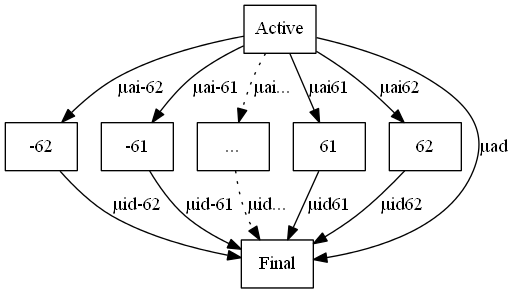
\includegraphics[scale=0.5]{gf810.png}
\caption{Markov-model for the parallelized GF810 Artificial Collective Spouse Pension plan.\label{fig:gf810}}
\end{figure}
\newcommand*{\diff}{\ensuremath{\mathit{diff}}}
The transition probability to one of the intermediary states $\mu_{ai}$ is the mortality intensity for the insured at time $t + age$ times the marriage probability that a $t + age$ year old is married to a $t + age + \diff$ year old with $\diff$ being the age difference between the spouse and the insured, as well as the number of the state.
The insured to final state $\mu_{ad}$ probability is the mortality intensity of the insured at time $t + age$ times the probability that the insured is not married at time $t + age$ (1 minus the marriage probability at the time).
The intermediary to final state $\mu_{id}$ probability is the mortality intensity of the spouse at the time (assuming the sexuality of the insured does not change) of age $t + age + \diff$.

This does potentially lead to a lot of cases where the insured will either be married to someone yet to be born or someone significantly older than the oldest person alive today, which can be a problem for the Gompertz-Makeham mortality intensity methods.
To lessen the impact of this, the result of these functions is constrained to be no higher than two by adding a constraint method.

This model of calculation can already be expressed in CalcSpec as is, but is somewhat cumbersome to write as there is little variability in the model.
The final CalcSpec should resemble code sample \ref{gf810cs}.
Note that the \lstinline$\var.expr$ is CalcSpec syntax for lambdas. 
It is currently also required to update the $from$ value in the $range$ section to the value of 120-age, as it is not currently possible to use variable values such as this in the current solution.
\clearpage
\begin{lstlisting}[language=calcspec, caption=GF810 full CalcSpec, label=gf810cs]
calculation = {
  name = "GF810 - Collective spouse pension", 
  algorithm = { type="Runge Kutta 4", parameters={ stepsize = 0.01 }}, 
  equations = { 
    0 = { r_j = rate, b_j = 0, mu_jk = { 
        1 = mu_ai(-62),
        2 = mu_ai(-61),
        ...,
        124 = mu_ai(61), 
        125 = mu_ai(62), 
        126 = \t.(GM_f(t)) * (1 - gp(t + age))
      }, b_jk = {  } }, 
    1 = { r_j = rate, b_j = 1, mu_jk = { 126 = mu_id(-62) }, b_jk = {}}, 
    2 = { r_j = rate, b_j = 1, mu_jk = { 126 = mu_id(-61) }, b_jk = {}}, 
    ...,
    124 = { r_j = rate, b_j = 1, mu_jk = { 126 = mu_id(61) }, b_jk = {}}, 
    125 = { r_j = rate, b_j = 1, mu_jk = { 126 = mu_id(62) }, b_jk = {}}, 
    126 = {  } }, 
  range = { from = 85, to = 0 }, 
  boundaryvalues = { 0 = 0, 1 = 0 }, 
  expressions = { 
    interestrate = 0.05, 
    age = 35, 
    rate(t) = interestrate, 
    GM_f(t) = constrain(0.0005 + 10 ^ (5.728 - 10 + 0.038 * (age + t))), 
    GM_m(t) = constrain(0.0005 + 10 ^ (5.88 - 10 + 0.038 * (age + t))), 
    mu_ai = \diff.\t.GM_f(t) * gp(t+age) * (h(t+age+diff)(t+age)), 
    mu_id = \diff.\t.GM_m(t + diff) 
  }
}
\end{lstlisting}

To optimize this process, functionality was added to transform the CalcSpec AST based on the variability of the GF810 plan.
See code sample \ref{gf810simplifiedcs} for an example of this which is converted back to the code in code sample \ref{gf810cs}.
%\clearpage
\begin{lstlisting}[language=calcspec, caption=GF810 simplified CalcSpec, label=gf810simplifiedcs]
calculation = { 
  name = "GF810 - Collective spouse pension", 
  algorithm = { type="Runge Kutta 4", parameters={ stepsize = 0.01 }}, 
  equations = { 
    GF810 = { age=age, rate=rate, mu_insured=GM_f, mu_spouse=GM_m }
  }, 
  range = { from = 85, to = 0 }, 
  boundaryvalues = { 0 = 0, 1 = 0 }, 
  expressions = { 
    interestrate = 0.05,
    age = 35,
    rate(t) = interestrate,
    GM_f(t) = constrain(0.0005 + (10 ^ (5.728 - 10 + 0.038 * (age + t)))),
    GM_m(t) = constrain(0.0005 + (10 ^ (5.88 - 10 + 0.038 * (age + t))))
  }
}
\end{lstlisting}

\subsubsection{Issues}
When attempting to compile the generated kernel with Alea.cuBase, an unexpected stack overflow exception was thrown during kernel compilation by Alea.cuBase.
By reducing the range of intermediary states from -62...+62 to -24...+24 for double precision and -36...+36 for single precision it was compilable again.

Various changes were made hoping to increase the maximum number of intermediary states but to no avail.
They consisted of the following:
\begin{itemize}
\item Reducing the depth of the generated AST. This included using a sum variable for the various state transitions as well as expression reduction by the $optimize$ method described in section \ref{subsec:exprReduction}.
\item Reducing the local memory used by moving the temporary arrays to shared memory.
\end{itemize}

\subsubsection{Results}
As the Alea.cuBase solution did not support the required number of states, a CPU-version was implemented to test the validity of the new method.
For age 35 it provided identical results down to the 7th decimal and as a bonus it completed in 1060 ms on average - an improvement of close to factor 150 compared to the original implementation.
Another interesting fact is that for age 35, the limited 50-states Alea.cuBase solution with intermediary states from -24...+24 was also identical down to the 7th decimal, and to the 10th decimal compared to the -62...+62 CPU version.
The sum of the reserve at every year also only leaves a relative difference of about 0.02\%, while the final result (year zero) only has an difference in results of $1.08794 \cdot 10^{-8}$ which is a relative error of no more than factor $9.733 \cdot 10^{-9}$.
The relative difference of the sum of the reserves for the CPU version with all intermediary states staying under 0.09\% for ages tested up to 80, with the final result difference not exceeding $1.2535 \cdot 10^{-7}$ which is a relative error not exceeding factor $6.107 \cdot 10^{-8}$.

This is sadly not a feat the limited 50-states implementation can claim to achieve. 
With age 15 there is a 9.45\% relative difference in the final result while at age 50 there is a 68.34\% relative difference.
For a visualization of this, see figure \ref{fig:gf810ages}. 
Note that many of the entries can not be seen as they are overlapping due to being practically identical.
The cause of the results getting progressively worse as the age increases is due to the fact that the marriage-probability in the early years is incredibly small.
It is also because as the insured grows older, the younger spouses account for a lot more of the reserve than older spouses that die earlier.
Since there are not enough intermediary states to reach these young spouses, the results are skewed.

\begin{figure}[h!]\centering
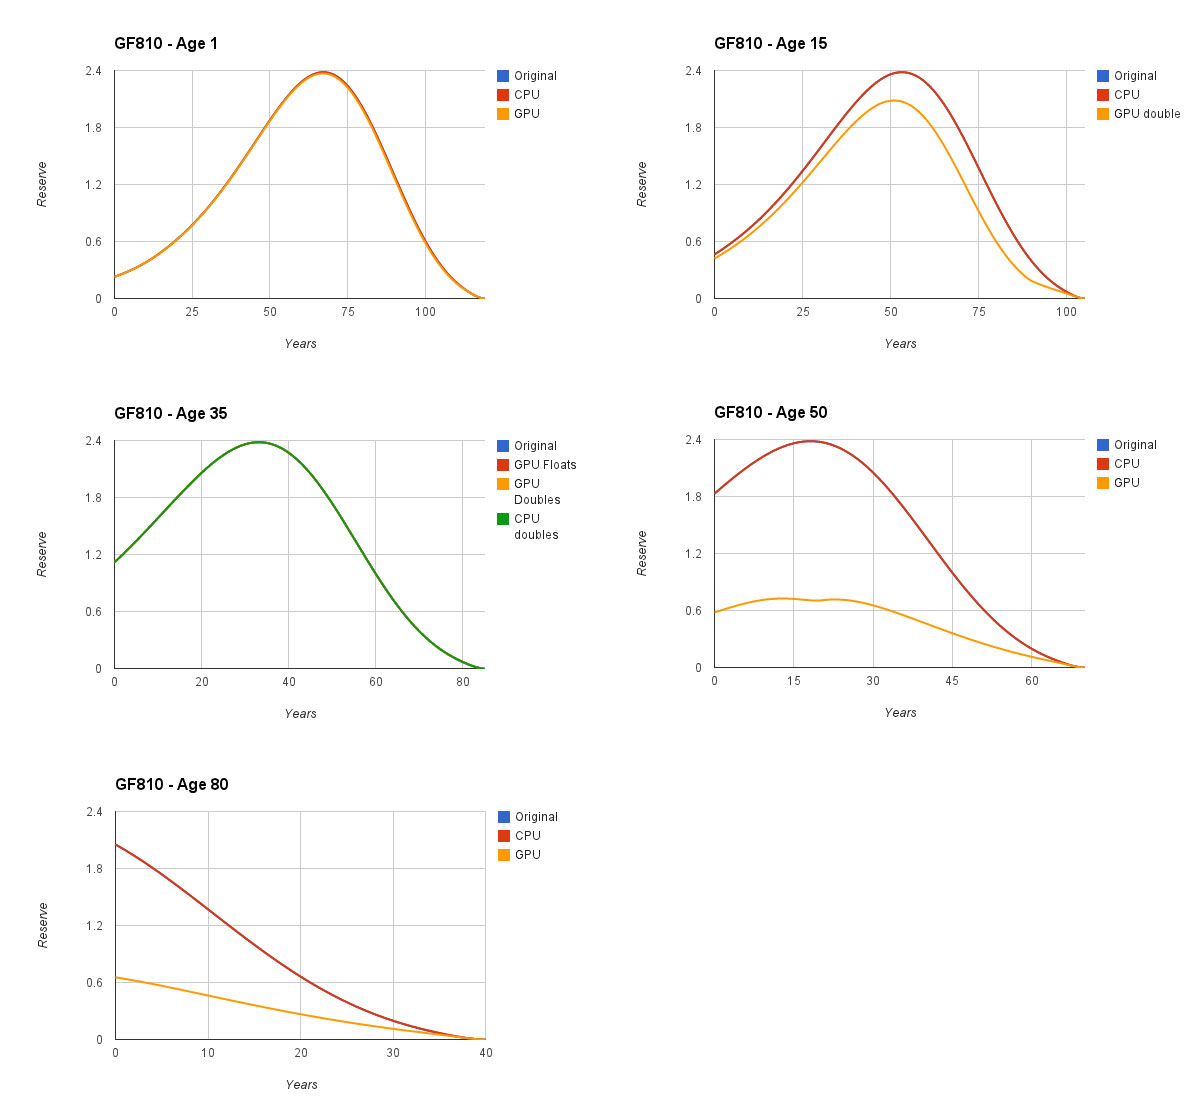
\includegraphics[scale=0.3]{GF810-ages.jpg}
\caption{Comparison of GF810 reserve-output for ages 1, 15, 35, 50 and 80 using results from the original solution, a CPU-version of the new method and the limited state GPU-version of the new method.\label{fig:gf810ages}}
\end{figure}

To conclude, the method definitely works in theory even if not currently on the GPU.
It does require all the intermediary states unless certain ``sweet spots'' are hit, which can not be relied upon.

Speed-wise, it is hard to compare running-times without being able to utilize all the required states.
For the limited 50-states version with intermediary states from -24...+24, tests were performed in section \ref{subsec:sharedmem} which resulted in runtimes of 5.52 seconds using global memory, 3.97 seconds using volatile shared memory and 4.30 second using non-volatile shared memory, but especially the shared memory results are inaccurate for the full solution as there is simply not enough shared memory available for all states.
If not using shared memory (or at least no more than 96 bytes per thread), 512 threads per block would still be an option.
This would result in the remaining registers spilling to local memory which would decrease performance.
An optimist could claim that similar relative increases as seen in simpler plans could be achieved, which would still be a massive performance increase.
A pessimist could argue that the use of slow local memory and overall complexity would limit the performance significantly.
No matter which camp you might be in, it is very likely that given enough iterations there should still be a significant increase in performance when calculating a large enough number of iterations.

For double precision comparison results, see appendix \ref{app:gf810ageresults}.

\subsubsection{Preliminary GPU performance exploration}
As the GF810 model uses many states and as a consequence consumes a lot of memory, it begs to question what limits this imposes.
When only using local memory, up to 512 threads per block remains an option.
This however requires a significant amount of memory and may not be efficient.

The current limited GPU version uses 50 states and not the ideal 126.
For age 35, where the calculation range of the Runge-Kutta four solver (see section \ref{subsec:background:thielerungekutta}) is from year 85 (120-age) to 0, with double precision floats it has a memory usage of 63 registers and 2696 bytes of local memory per thread.
Increasing the number of states by one should in theory only affect the temporary arrays of the Runge-Kutta four solver, leading to an increase in local memory usage by 40 bytes for double precision floats (one more state in six temporary arrays times eight bytes for double precision floats).
This would result in the total amount of memory used for age 35 with double precision $(126 - 50) * 40 + 2696 = 5736$ bytes per thread, or at most $5736 * 512 * 14 = 41115648$ bytes (39.21 MiB) concurrent memory usage with 512 threads and all SMs running a block.
Testing showed that increasing the number of states by one increased the memory usage by more than 40, ranging from 40 to 57.5 bytes per state, but this might increase further for higher numbers of states.
Assuming a worst case of 58 bytes per state, the total memory consumption per thread would reach 7104 and concurrent memory usage would peak at about 48.56 MiB.
Other sources of memory usage include the result array stored in global memory which for age 35 would use up to $86 * 126 * 512 * 8 = 44384256$ bytes (42.33 MiB) per block with 512 threads per block.
Assuming a practical minimum of 14 blocks, this leads to a total concurrent GPU memory usage of 613.8MiB, a significant amount less than the 4GiB available global memory.

Working with large amounts of memory can also lead to potential problems for the CPU.
While compilation to x64 should allow for array sizes of up to 2,147,483,647 as arrays use an integer for indexing, and while the result array is still using significantly less memory than the 2GiB x64 single object restriction of the .NET Common Language Runtime, out of memory-errors were encountered on the test machine when allocating device memory and gathering the results from the GPU, potentially because of the relatively small amount of CPU RAM (4GiB).
This limited the range of the following performance tests.

The high memory throughput of the GF810 plan potentially gives it other properties than the simpler life insurance plans.
To discover what launch configuration are most efficient at high memory throughput is not so clear, but tests were performed to provide some insight despite only being done with a limited number of states.
See table \ref{table:gf810gpuperformance} for the main results of the test, and see appendix \ref{app:gf810performance} for all the test results.
Do note that it uses iterations per second rather than per millisecond as seen in previous tables due to the increased computational complexity.
The hypothesis that it is inefficient to use less than 14 blocks or 32 threads per block is reconfirmed even at high memory throughput.
See the rows of the table with launch parameters (7,512), (224, 16), (1, 32) and (1, 1) for examples of this.
The majority of the remaining launch parameters used no more than 3584 iterations (for example the launch parameters with 112 blocks and 32 threads per block) due to previously mentioned memory problems, but with varying levels of performance.
It seems that due to the high memory throughput it is preferable to increase the number of blocks over threads as long as at least 32 threads per block (a warp) is used.
Knowing that it seems most efficient at just one warp means that multiple launches of the kernel is a possibility that could limit the size of the result array.
That does mean that functionality to skew the scope of the launch would have to be added.
Alternatively, as long as there is total faith in the results, only the final result of the first state in year 0 is typically required, eliminating memory issues when gathering the results from the GPU.

\begin{table}[h!]
\centering
{\setlength{\extrarowheight}{2pt}{\setlength{\tabcolsep}{3pt}
\begin{tabular}{ | l | r | r | }
  \hline
Launch parameters	&	Kernel time	&	Iterations per second	\\ \hline
(1, 1)				&	4.95		&	0.2						\\ \hline
(1, 32)				&	4.84		&	6.61					\\ \hline
(7, 512)			&	11.80		&	303.93					\\ \hline
(14, 32)			&	6.74		&	66.50					\\ \hline
(14, 128)			&	8.08		&	221.87					\\ \hline
(14, 256)			&	11.68		&	306.76					\\ \hline
(28, 128)			&	10.68		&	335.69					\\ \hline
(56, 64)			&	9.51		&	376.69					\\ \hline
(112, 32)			&	9.43		&	379.90					\\ \hline
(224, 16)			&	20.49		&	174.89					\\ \hline
\end{tabular}}}
\caption{Limited GF810 with age 35 GPU performance explorations with various launch parameters.\label{table:gf810gpuperformance}}
\caption*{Launch parameters are of the form (blocks, threads per block). Kernel time is in seconds.}
\end{table}

\subsubsection{Step-size experimentation}
A straight-forward way to increase performance is to reduce the number of steps used by the Runge-Kutta solver at the cost of increased error.
This was tested on the CPU-implementation of the new GF810 method with 16, 32 and 64 as the number of steps compared to the original 100 steps, and tested for ages 10 to 100 in 5 year intervals.
Similar relative performance impacts should be seen on the GPU.

Results showed that with just 16 steps an average relative error compared to 100 steps was no more than $6.18318 * 10^{-11}$ with an increase in performance of factor 6.24.
When using 32 steps, the error was reduced to $6.3476 * 10^{-12}$ with an increase in performance of factor 3.13, and with 64 as the number of steps, the error was reduced to $1.626 * 10^{-12}$ with an increase in performance by factor 1.57.

One important trend to note is the fact that as age increases, and as a result the years calculated decreases, the rate of error increases.
As the high-age calculations already require less computation it would be ideal to use a larger number of steps for these computations.

For the results of the various step-sizes, see appendix \ref{app:gf810stepsizes}.


	\section{Related Work}
Related work, include Dahl+Harrington for sure
	% !TeX root = ../thesis.tex
\section{Future Work}
There is much potential future work that could be done, some of which has been mentioned briefly already.
For example, the manual parameterized implementation of the life insurance plans seen in section \ref{sub:manual_parameterization} showed almost a doubling of performing with double precision floats compared to CUDA C and subsequently the parameterized CalcSpec-generated life insurance plans.
The main difference is the fact that parameters such as age and interest rate were passed down as method parameters and it was speculated that the difference in speed was due to this, but as of yet it is untested.

There are also minor improvements that could be made for CalcSpec such as variables being made usable in the \lstinline$range$ section of CalcSpec and respecting the values in \lstinline$output$ and \lstinline$boundaryvalues$.
The current type system used during conversion of CalcSpec to quotations is also too simplistic and does not natively support multi-parameter methods requiring hacks to support methods such as $\mu_{ai}$ and $\mu_{id}$ seen in section \ref{subsubsec:gf810parallelized}.
The limitations of the current type systems also makes implementing the parameter passing difficult.
There are also many limitations on how the \lstinline$delta$ method (see section \ref{subsec:delta}) can be used.
These are not all currently being checked, nor are the requirements communicated very well.

The expression reduction seen in section \ref{subsec:exprReduction} was also shown to have a small impact on performance but is still very simplistic, and more work could likely be done to even greater effect.

If not fixed by the authors of Alea.cuBase QuantAlea, work should be done to allow for more states, ensuring that complex plans such as the GF810 plan mentioned in section \ref{sub:gf810} can be used.
When possible, performance implications of various types of memory should also be tested.
Alternatively, the intermediary states can be skewed so rather than going from -24...+24 it could go from -38...10 to prioritize the ``expensive´´ spouses that account for the majority of the reserve.
This should also take into account the age of the insured, so that no intermediary states are ``wasted''.

Variable shared memory also looks interesting. For low-register plans shared memory seems to be a detriment to the performance, but as an alternative to local memory it is much preferable.
Shared memory is however a limited resource and it is especially limited by the number of states in the life insurance model.
Intelligently selecting elements of the Runge-Kutta 4 solver to be moved to shared memory should provide a respectable increase in performance.

An interesting prospect would be moving the architecture to the cloud.
This would allow for parallelization utilizing multiple virtualized GPUs on an on-demand basis lessening the capital investment needed for intense parallel computing.
Whether the current cloud providers provide adequate virtualized GPU instances is the question and the performance impact is of great interest.

\section{Conclusion}
In this project a single-threaded C\# implementation of a Runge-Kutta 4 solver as well as six example life insurance plans (see section \ref{subsec:initialsolution}) has been transformed to utilize parallelization on the CUDA platform.
Furthermore, the Actulus Calculation Specification (CalcSpec, see section \ref{subsec:background:calcspec}) for life insurance products was made directly transformable into GPU code using F\# and Alea.cuBase (see section \ref{subsec:background:fsharpcubase} and \ref{sec:calcspecgeneration}).
Finally, the collective spouse pension (GF810, see section \ref{sub:gf810}) was improved by using a new calculation method by Klaus Grue which resulted in a performance increase of factor 150.

The performance for single precision floats was up to 2485 faster for the parameterized CalcSpec generated life insurance plans.
For double precision floats an improvement of factor 1335 was measured in the manual parameterized implementation while the CalcSpec generated implementation managed an improvement of factor 634.

Alea.cuBase, F\# and .NET as platforms have had little or no negative performance impact (seemingly quite the contrary) and has allowed for significantly more flexible GPU kernels by utilizing runtime-compilation of kernels.
This means that it is more than viable and a good alternative to CUDA C for life insurance policy parallelization.
The kernels are highly optimized by Alea.cuBase but did show improvements from being optimized locally using expression reduction.
There are however some as of yet unsolved problems with Alea.cuBase as the provided methods for limiting registers in kernels did not work, and working with larger state models such as the GF810 collective spouse pension threw a stack overflow exception during kernel compilation for unknown reasons.

\clearpage
	
	
	\bibliography{sections/Bibliography}
    \clearpage
	\appendix
	\addappheadtotoc
	% !TeX root = ../thesis.tex
%\begin{appendices}
  % !TeX root = ../../thesis.tex
\section{Results of running deviceQuery}\label{app:deviceQuery}
\RecustomVerbatimCommand{\VerbatimInput}{VerbatimInput}%
{fontsize=\footnotesize,
 %
 frame=lines,  % top and bottom rule only
 framesep=2em, % separation between frame and text
 commandchars=\|\(\), % escape character and argument delimiters for
                      % commands within the verbatim
 commentchar=*        % comment character
}
\VerbatimInput{sections/appendix/deviceQuery.txt}
  % !TeX root = ../../thesis.tex
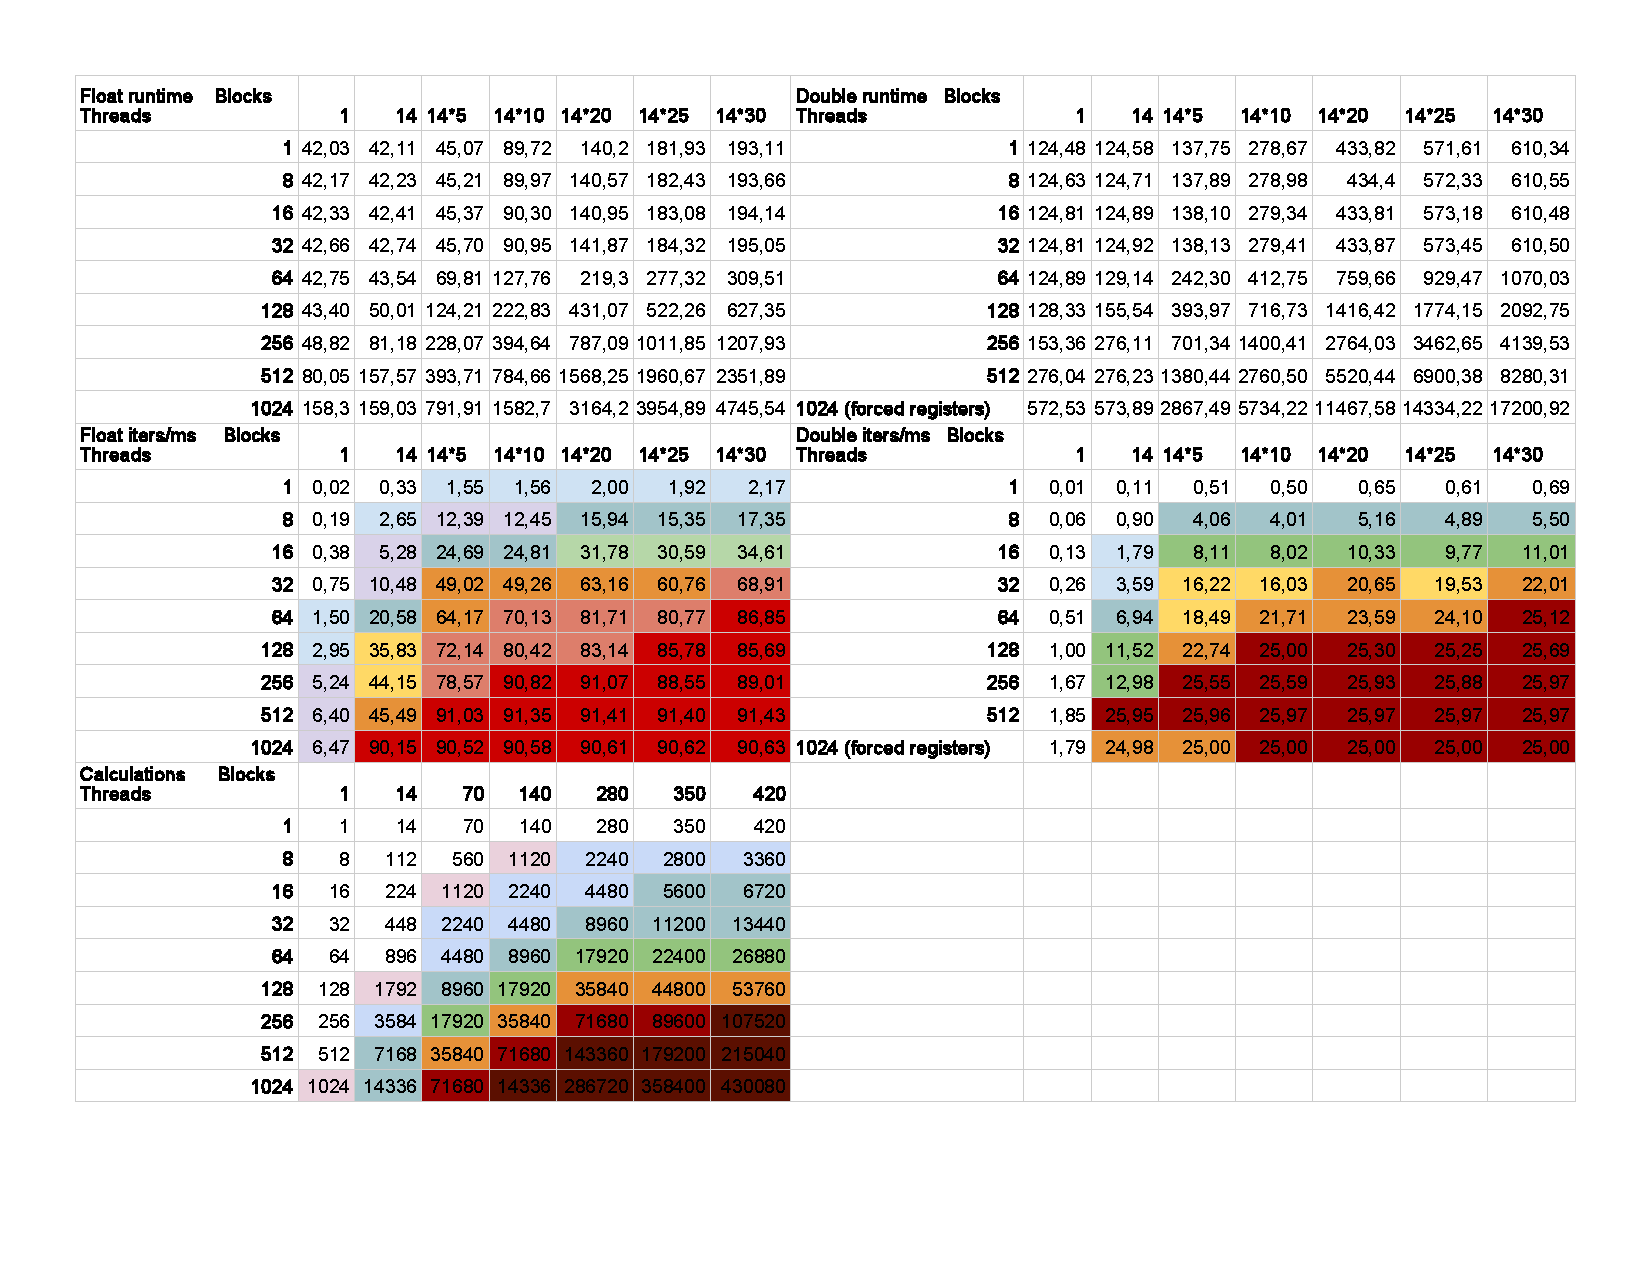
\includepdf[pages=1,angle=90,pagecommand={\section{CUDA C Performance Test}\label{app:cuda_runtimes}}, frame,scale=0.65]{sections/appendix/cuda_runtimes.pdf}
%\end{appendices}
\end{document}